\documentclass{homework}

\title{Tarea 4}
\date{2020-05-01}
\gdate{1er Semestre 2020}
\author{Nicholas Mc-Donnell}
\course{Geometría Diferencial - MAT2305}

\setkeys{Gin}{width=.9\textwidth}

\begin{document}
\maketitle
\newpage
\pagenumbering{arabic}

\begin{sol}[1]
    Se calculan las siguientes cosas:
    \begin{align*}
        \vec{x}_u&=(1-u^2+v^2,2uv,2u)\\
        \vec{x}_v&=(1+u^2-v^2,2uv,-2v)\\
        \vec{x}_{uu}&=(-2u,2v,2)\\
        \vec{x}_{uv}&=(2v,2u,0)\\
        \vec{x}_{uu}&=(2u,-2v,-2)\\
    \end{align*}
    \begin{enumerate}
        \item Para calcular los coeficientes de la primera forma fundamental se ven las siguientes relaciones:
        \begin{align*}
            E&=\angled{\vec{x}_u,\vec{x}_u}\\
            F&=\angled{\vec{x}_u,\vec{x}_v}\\
            G&=\angled{\vec{x}_v,\vec{x}_v}
        \end{align*}
        Haciendo unos cálculos\footnote{Están en el apendice.} y viendo simetrías, se llega a que:
        \begin{align*}
            E&=(1+u^2+v^2)^2\\
            F&=0\\
            G&=(1+u^2+v^2)^2\\
        \end{align*}
        \item Para calcular los coeficientes de la segunda forma fundamental se calcula\footnote{Ver 1.} \(N\):
        \begin{equation}
            N=\frac1{(1+u^2+v^2)^2}\paren{-2u,2v,1-u^2-v^2}
        \end{equation}
        Y usando las siguientes relaciones se calculan los coeficientes de la segunda forma fundamental\footnote{Ver 1.}:
        \begin{align*}
            e&=\angled{N,\vec{x}_{uu}}\\
            f&=\angled{N,\vec{x}_{uv}}\\
            g&=\angled{N,\vec{x}_{vv}}\\
        \end{align*}
        Y usando el hecho de que \(\vec{x}_{uu}=-\vec{x}_{vv}\) se llega a que:
        \begin{align*}
            e&=2\\
            f&=0\\
            g&=-2\\
        \end{align*}
        \item Sean \(\alpha(u)=\vec{x}(u,v_0)\) y \(\beta(v)=\vec{x}(u_0,v)\) curvas coordenadas, luego \(\alpha'(u)=\vec{x}_u(u,v_0)\) y \(\beta'(v)=\vec{x}_v(u_0,v)\). Ahora, se usan las siguientes relaciones para calcular \(\d{N}\) en base \(\{\vec{x}_u,\vec{x}_v\}\):
        \begin{align*}
            a_{11}&=\frac{fF-eG}{EG-F^2}\\
            a_{12}&=\frac{gF-fG}{EG-F^2}\\
            a_{21}&=\frac{eF-fE}{EG-F^2}\\
            a_{22}&=\frac{fF-gE}{EG-F^2}\\
        \end{align*}
        Simplificando un poco se tiene que \(a_{11}=\frac{e}{E},a_{12}=a_{21}=0,a_{22}=\frac{g}{G}\), por lo que \(a_{11}=-a_{22}=\frac2{(u^2+v^2+1)^2}\). Con eso, se ve lo siguientes:
        \begin{equation*}
            \d{N}=\begin{pmatrix}
                a_{11}&0\\
                0&a_{22}
            \end{pmatrix}
        \end{equation*}
        Como \(\d{N}\vec{x}_u=a_{11}\vec{x}_u\) y \(\d{N}\vec{x}_v=a_{22}\vec{x}_v\) por definición, se usa el teorema de Olinde Rodrigues y se tiene que \(\alpha\) y \(\beta\) son lineas de curvaturas.
        \item Ahora se usa que \(K=\det(\d{N})\) y que \(H=-\frac12\tr(\d{N})\), con lo que se ve que \(K=\frac{-4}{(1+u^2+v^2)^4}\) y que \(H=0\). Por lo que \(X\) es superficie mínima, y como \(a_{11}=-a_{22}, K=a_{11}a_{22}\), se tiene que \(k_1=a_{11}\) y \(k_2=a_{22}\).
    \end{enumerate}
\end{sol}

\begin{sol}[2]
    Sea \(\vec{x}(u,v)=(u\cos(v),u\sin(v),(u-1)^3+1)\), con \(U=\{(u,v):0<u<2,0<v<2\pi\}\), se hacen unos cálculos\footnote{Ver 1.} y se llega a que:
    \begin{align*}
        a_{11}&=\frac{-6(u-1)}{\paren{9(u-1)^4+1}^{\frac32}}\\
        a_{22}&=\frac{-3(u-1)^2}{\sqrt{9(u-1)^4+1}}\\
        a_{12}&=a_{21}=0
    \end{align*}
    Luego, los puntos que corresponden al origen son los que cumplen que \(u=1\), ahora se ve lo siguiente:
    \begin{align*}
        K&=a_{11}a_{22}=0\\
        H&=-\frac12(a_{11}+a_{22})=0
    \end{align*}
    Por lo que son planares.
\end{sol}

\begin{sol}[3]
    Se toma el ejemplo \(X(u,v)=(u,v,u^4+2u^2v^2+v^2)\), se hacen varios cálculos\footnote{Ver 1.} y se llega a la siguiente expresión de la curvatura Gaussiana:
    \begin{equation*}
        K=\frac8{c^2}\cdot\frac{4v^4+4u^2v^2+3u^2+3v^2}{((4u(u^2+v^2))^2+1)((2v(u^2+1))^2+1)-4u(u^2+v^2)2v(u^2+1)}
    \end{equation*}
    Donde \(c=\norm{\vec{x}_u\wedge\vec{x}_v}=\sqrt{(4u(u^2+v^2))^2+(2v(v^2+1))^2+1}\), se nota que el denominador de \(K\) es de la forma \((a^2+1)(b^2+1)-ab=a^2+b^2-ab+a^2+b^2+1\), como \(a^2+b^2\geq ab\), se tiene que el denominador es estrictamente mayor a \(0\). Ahora, el numerador de \(K\) es mayor o igual a \(0\), más aún es igual a \(0\) ssi \(u=v=0\). Por lo que \((0,0)\) es el único punto parabólico de \(X\).
\end{sol}

\begin{sol}[4]
    \begin{enumerate}
        \item Sea \(S\) una superficie regular compacta, y sea \(\Gamma\) el conjunto de esferas con centro \(O\) tal que \(S\) está contenida en ellas. Se nota que existe un radio \(r\) ínfimo de estas esferas, sea \(\Sigma\) la esfera de radio \(r\) y centro \(O\), s.p.d.g. \(O\) es el origen y \(r=1\). Ahora, claramente \(\Sigma\cap S\neq\emptyset\), sea \(p\in\Sigma\cap S\), s.p.d.g. \(p=(0,0,-1)\). Luego, sea \(P\) el plano tangente a \(\Sigma\) en \(p\), entonces \(P\) es tangente a \(S\), porque \(P\) no puede contener más puntos de \(\Sigma\) además de \(p\) y \(S\) está contenida en \(\Sigma\). Ahora, como \(P\) es tangente a \(S\) y a \(\Sigma\), se tiene que \(S\) y \(\Sigma\) son tangentes en \(p\). Ahora, sea \(N\) un plano normal a \(P\) en \(p\), ahora existe un \(\varepsilon>0\) tal que
        \begin{align*}
            P\cap\Sigma&=\{R(x,0,\sqrt{1-x^2}):x\in(-\varepsilon,\varepsilon)\}\\
            P\cap S&=\{R(x,0,f(x)):x\in(-\varepsilon,\varepsilon)\}
        \end{align*}
        Donde \(R\) es una matriz de rotación y \(f\) es la parametrización de la curva correspondiente, se denota \(g(x)=\sqrt{1-x^2}\). Ahora, se tiene que \(k_{S,N}(p)\) es la curvatura normal de \(S\) del plano normal \(N\) en \(p\), más aún \(k_{S,N}(p)=f''(0)\)\footnote{Se tiene que la normal a la curva es proporcional a la normal a la superficie y \(k=f''(0)\)}. Dado esto, se ve que para \(x>0\) \(f\) es localmente creciente, más aún localmente \(f'(x)\geq g'(x)\), similarmente si \(x<0\) se tiene que localmente \(f'(x)\leq g'(x)\), por lo que si \(x<0<y\) se tiene que \(\frac{f'(y)-f'(x)}{y-x}\geq\frac{g'(y)-g'(x)}{y-x}\), como \(f''(0)\) y \(g''(0)\) existen al tomar el limite de \((x,y)\rightarrow(0,0)\) se llega a que \(f''(0)\geq g''(0)\), como \(g''(0)\) es la curvatura de \(\Sigma\) (una esfera) se tiene que \(g''(0)>0\), con lo que \(k_{S,N}(p)>0\) para todo plano normal, con lo que se tiene lo pedido.
        \item Por contradicción, se asume que existe una superficie \(S\) que cumple lo pedido, por la parte (a) existe un punto elíptico \(p\) en \(S\), por lo que s.p.d.g. \(k_1,k_2>0\) por lo que \(H(p)\neq0\), una contradicción.
    \end{enumerate}
\end{sol}

\begin{sol}[5]
    \begin{enumerate}
        \item 
        \item Sea \(f(x,y,z)=x^2+y^2-z^2\), luego \(X(U)=\{(x,y,z):f(x,y,z)=0\}\cap\{(x,y,z):0<z<1\}\). Se nota que la normal a \(X(U)\) en \(p\) \(N\) es igual a \((f_x,f_y,f_z)=\frac1{\sqrt{2}z}(x,y,-z)\), por lo que \(N(u,v)=\frac1{\sqrt{2}}(\cos v,\sin v, -1)\). Ahora, la curva \(C\subset X(U)\) donde \(z=z_0\) se puede parametrizar de la siguiente manera \(\vec{x}(v)=(z_0\cos v,z_0 \sin v, z_0)\), y como es un círculo su curvatura \(k\) corresponde a \(\frac1{z_0}\)\footnote{\(z_0\) es el radio del círculo.} y su normal en \(v\) es \((\cos v,\sin v, 0)\), con lo que \(k_n=\frac1{z_0\sqrt{2}}\).
        \item Se nota que dado un punto \(p\) en \(X(U)\) se puede construir una recta \(\alpha:(a,b)\rightarrow X(U)\) tal que \(\lim_{t\rightarrow a}\alpha(t)=\vec{0}\) y que para algún \(c\in(a,b)\) se tiene que \(\alpha(c)=p\). Se ve que los puntos de está curva son tangentes al mismo plano, por lo que se aplica (a) y se tiene que \(p\) es un punto parabólico o planar, pero \(p\) también pertenece a un círculo con \(z=z_0\) para algún \(z_0\), por lo que \(k_n\neq0\), con esto se tiene que \(p\) es un punto parabólico, como \(p\) es arbitrario todo los puntos de \(X(U)\) son parabólicos.
    \end{enumerate}
\end{sol}

\section*{Apéndice}
\begin{center}
    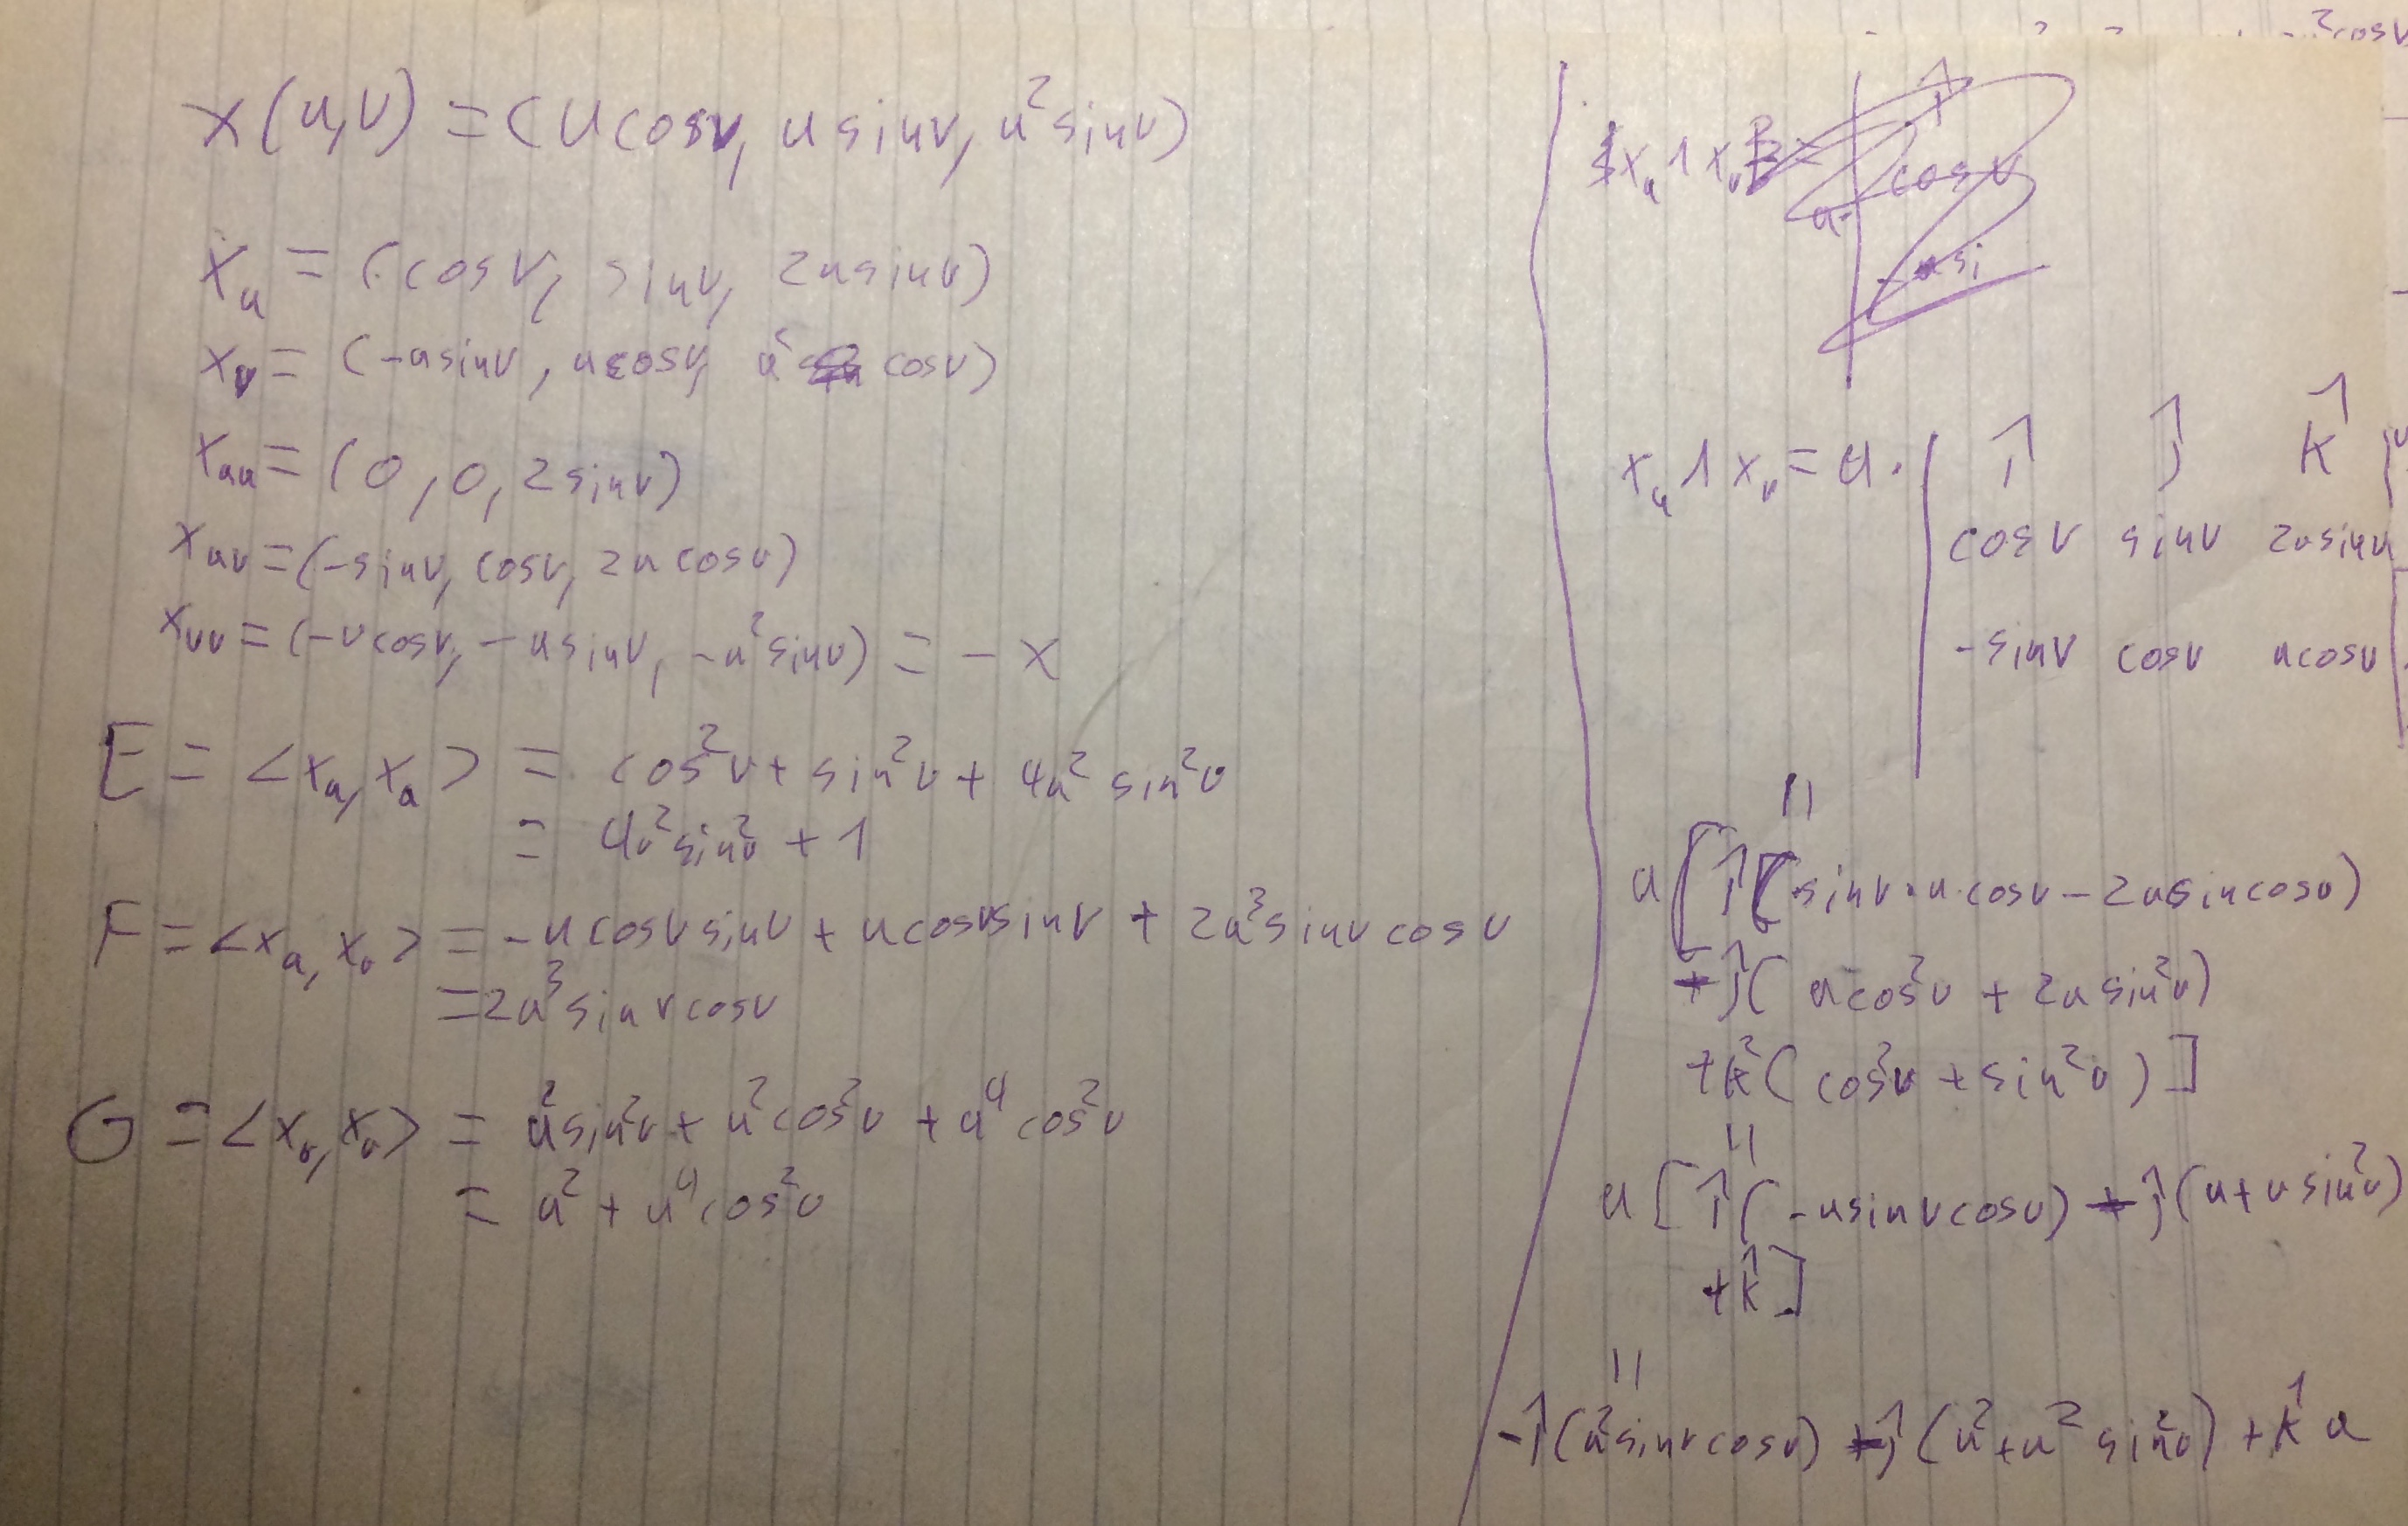
\includegraphics{img/IMG_5982.JPG}
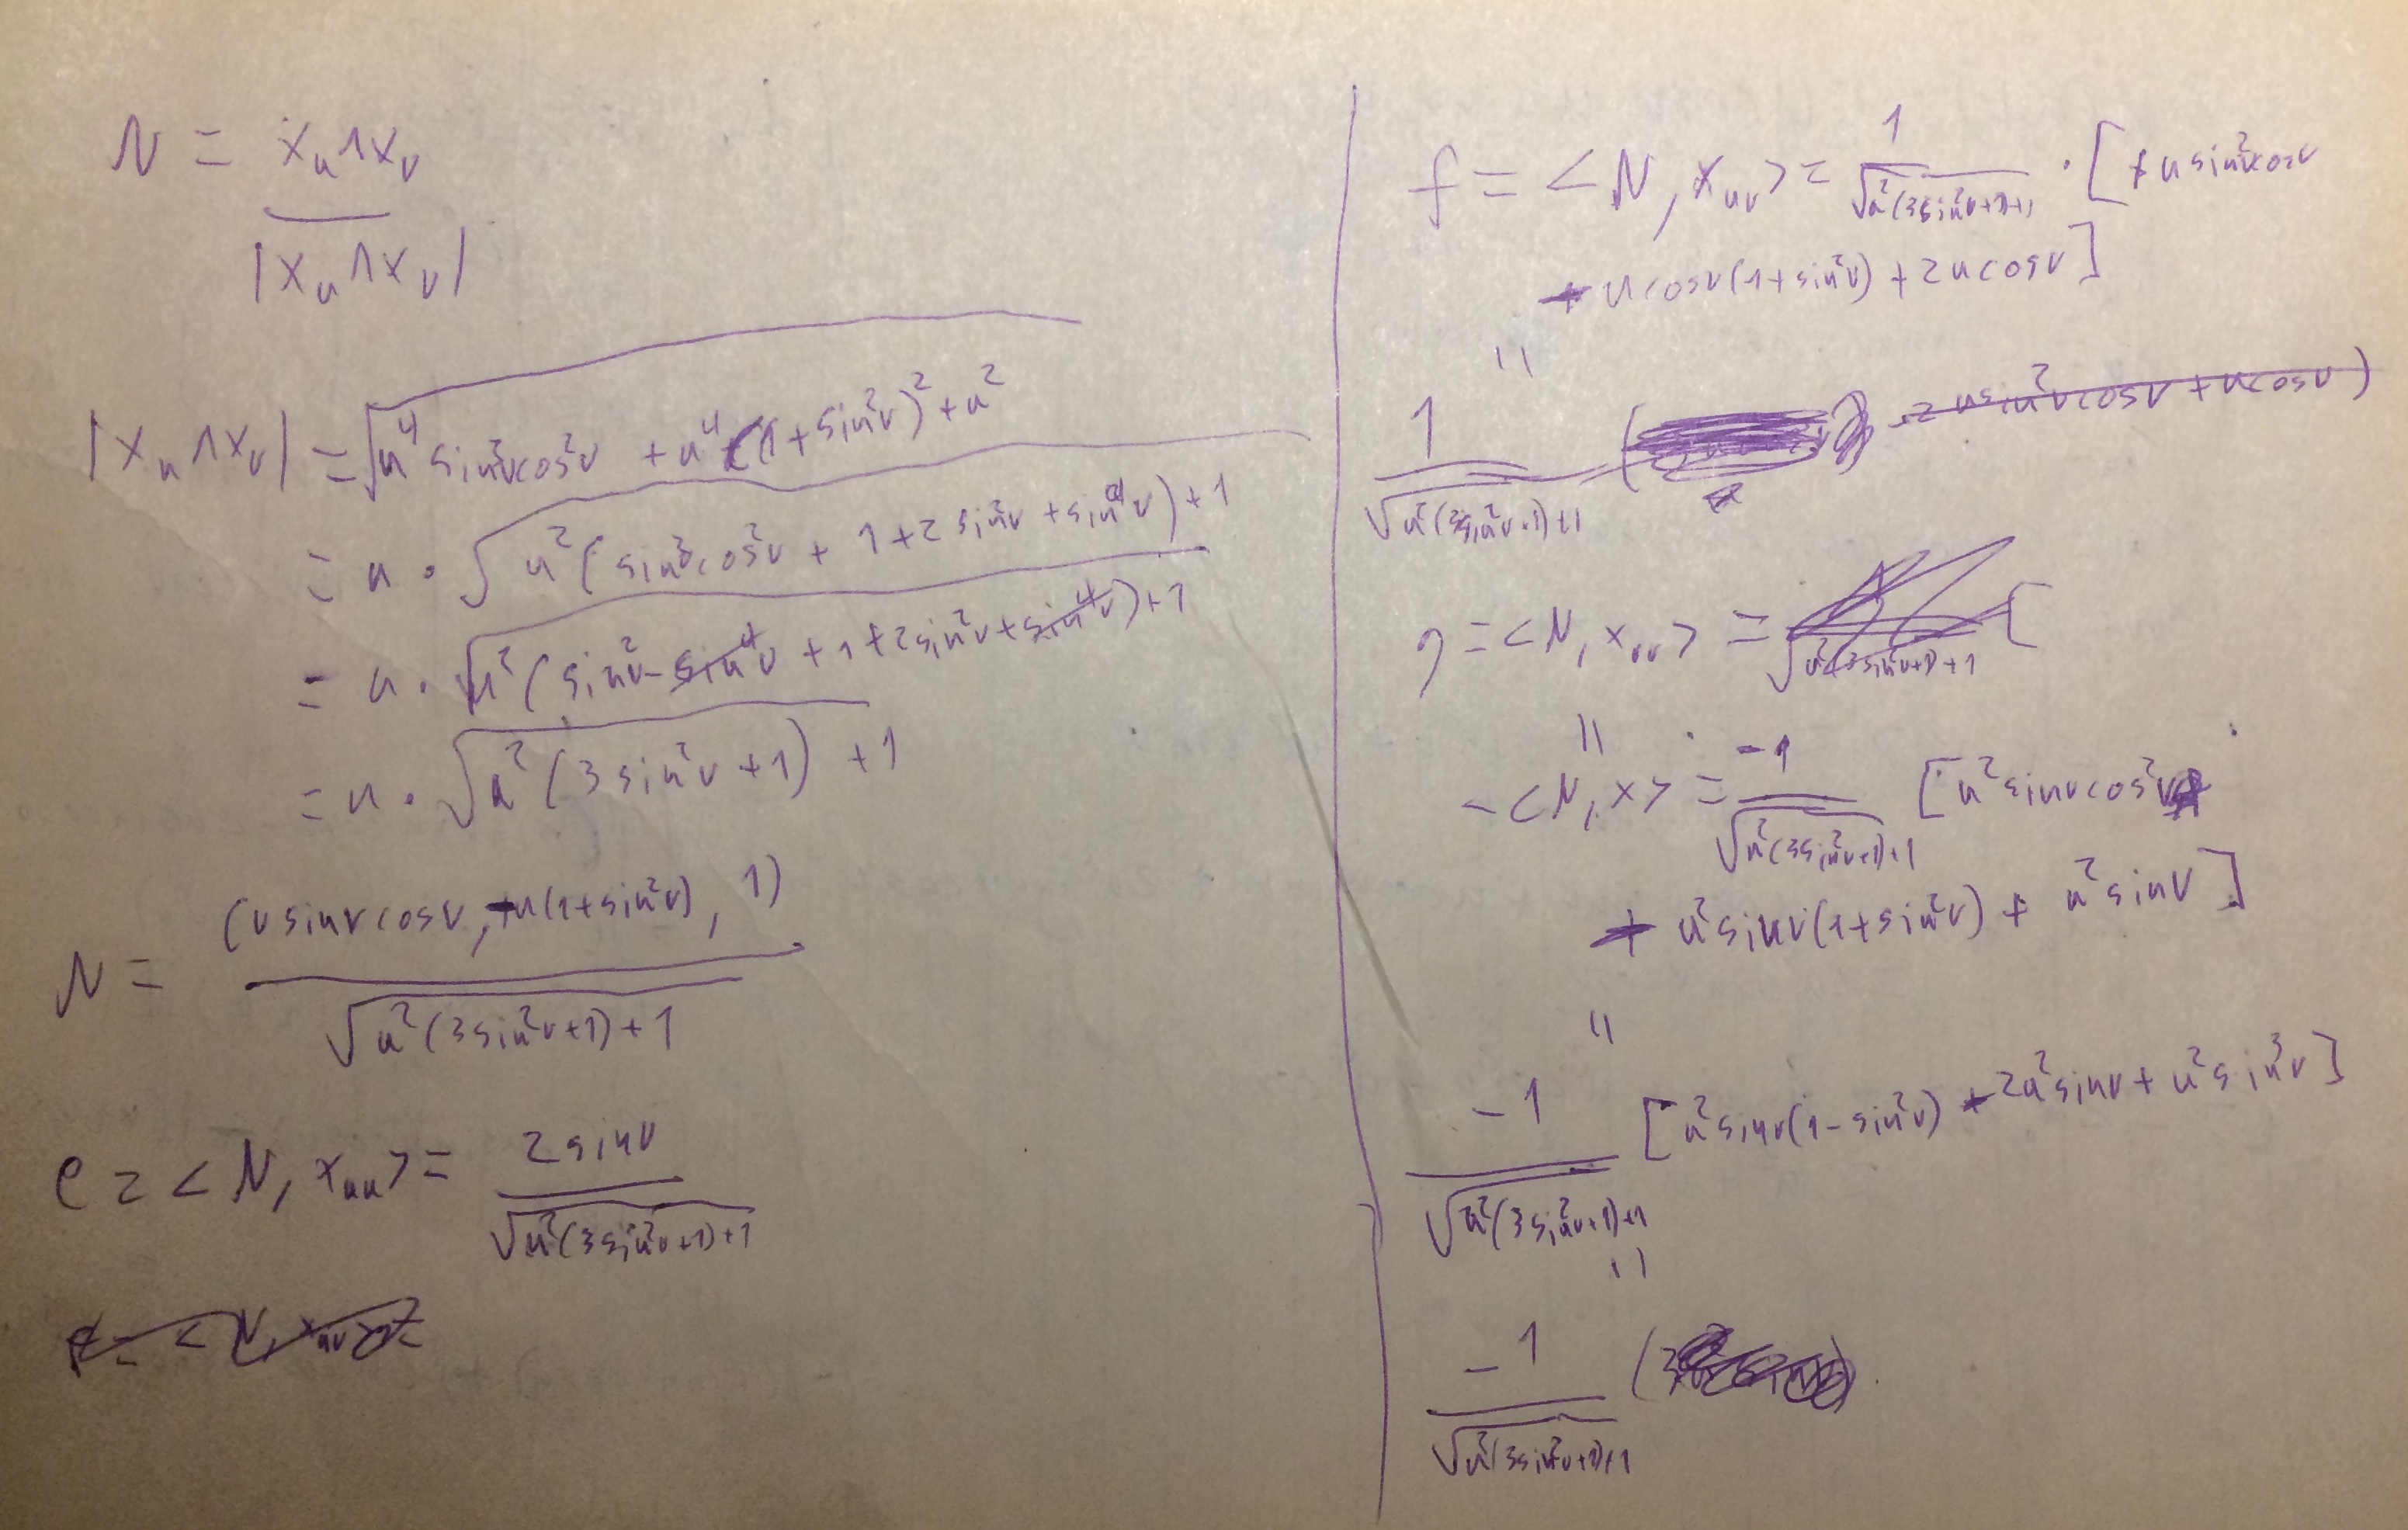
\includegraphics{img/IMG_5983.JPG}
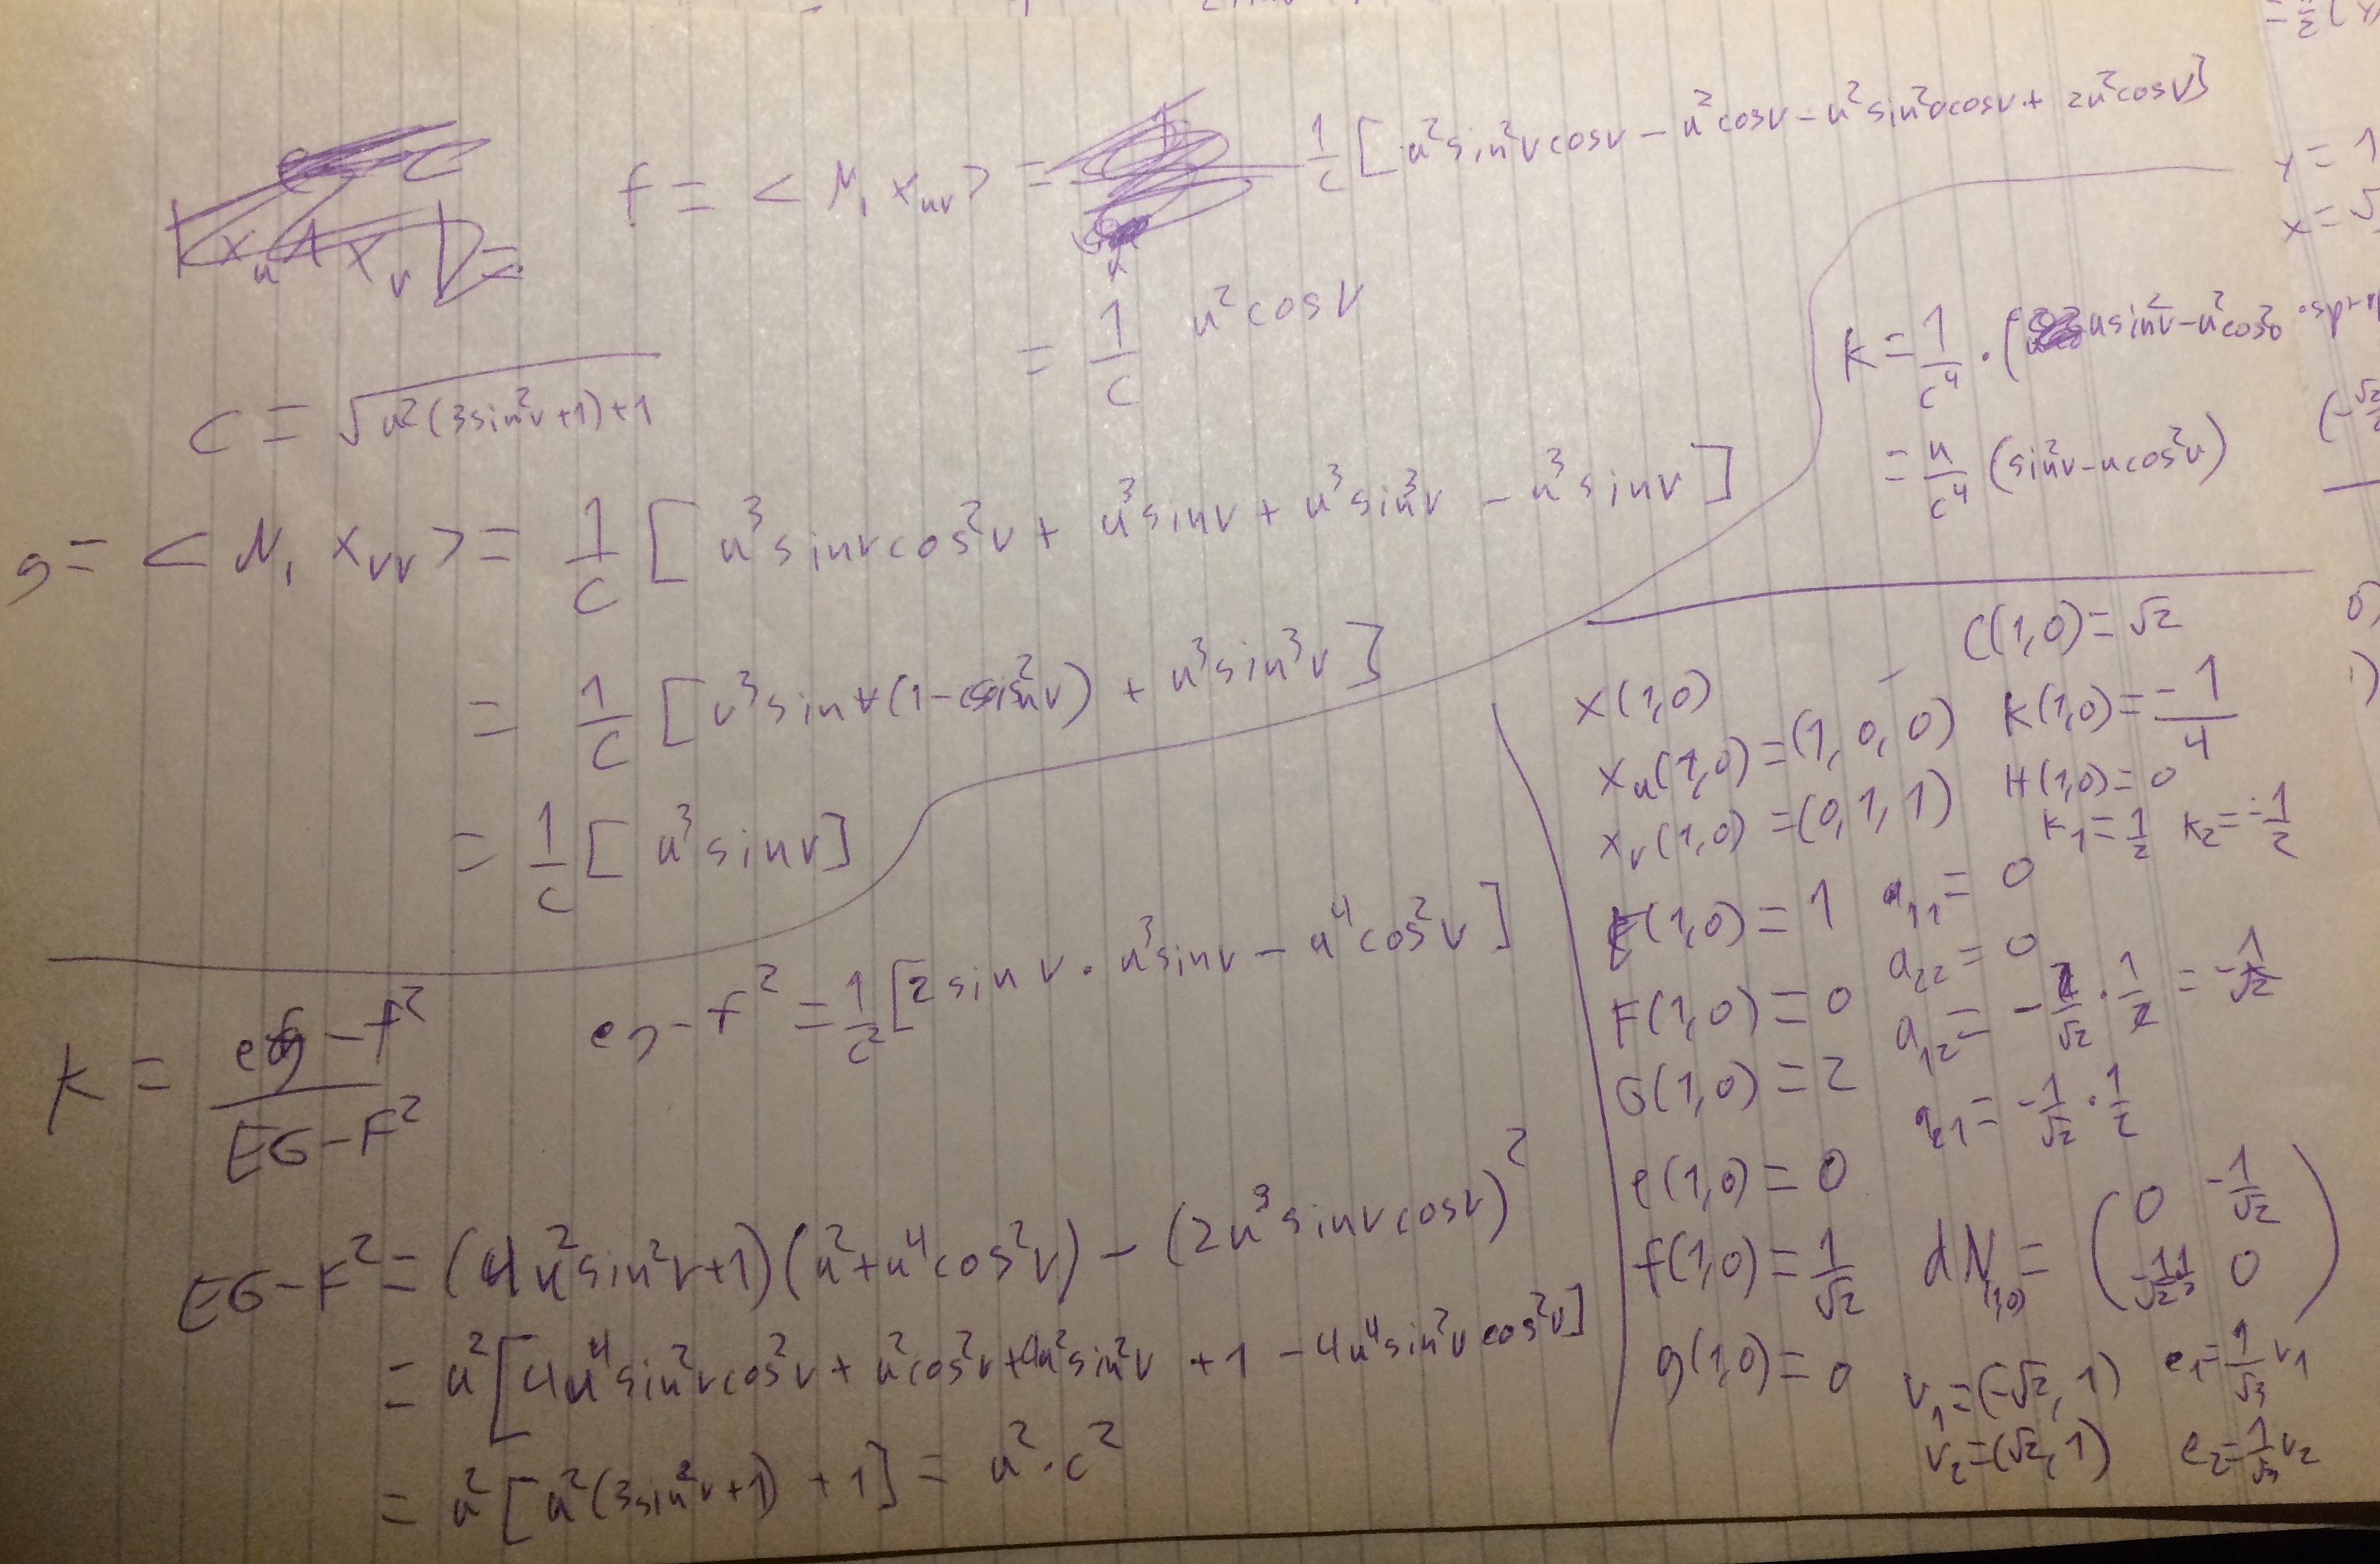
\includegraphics{img/IMG_5984.JPG}
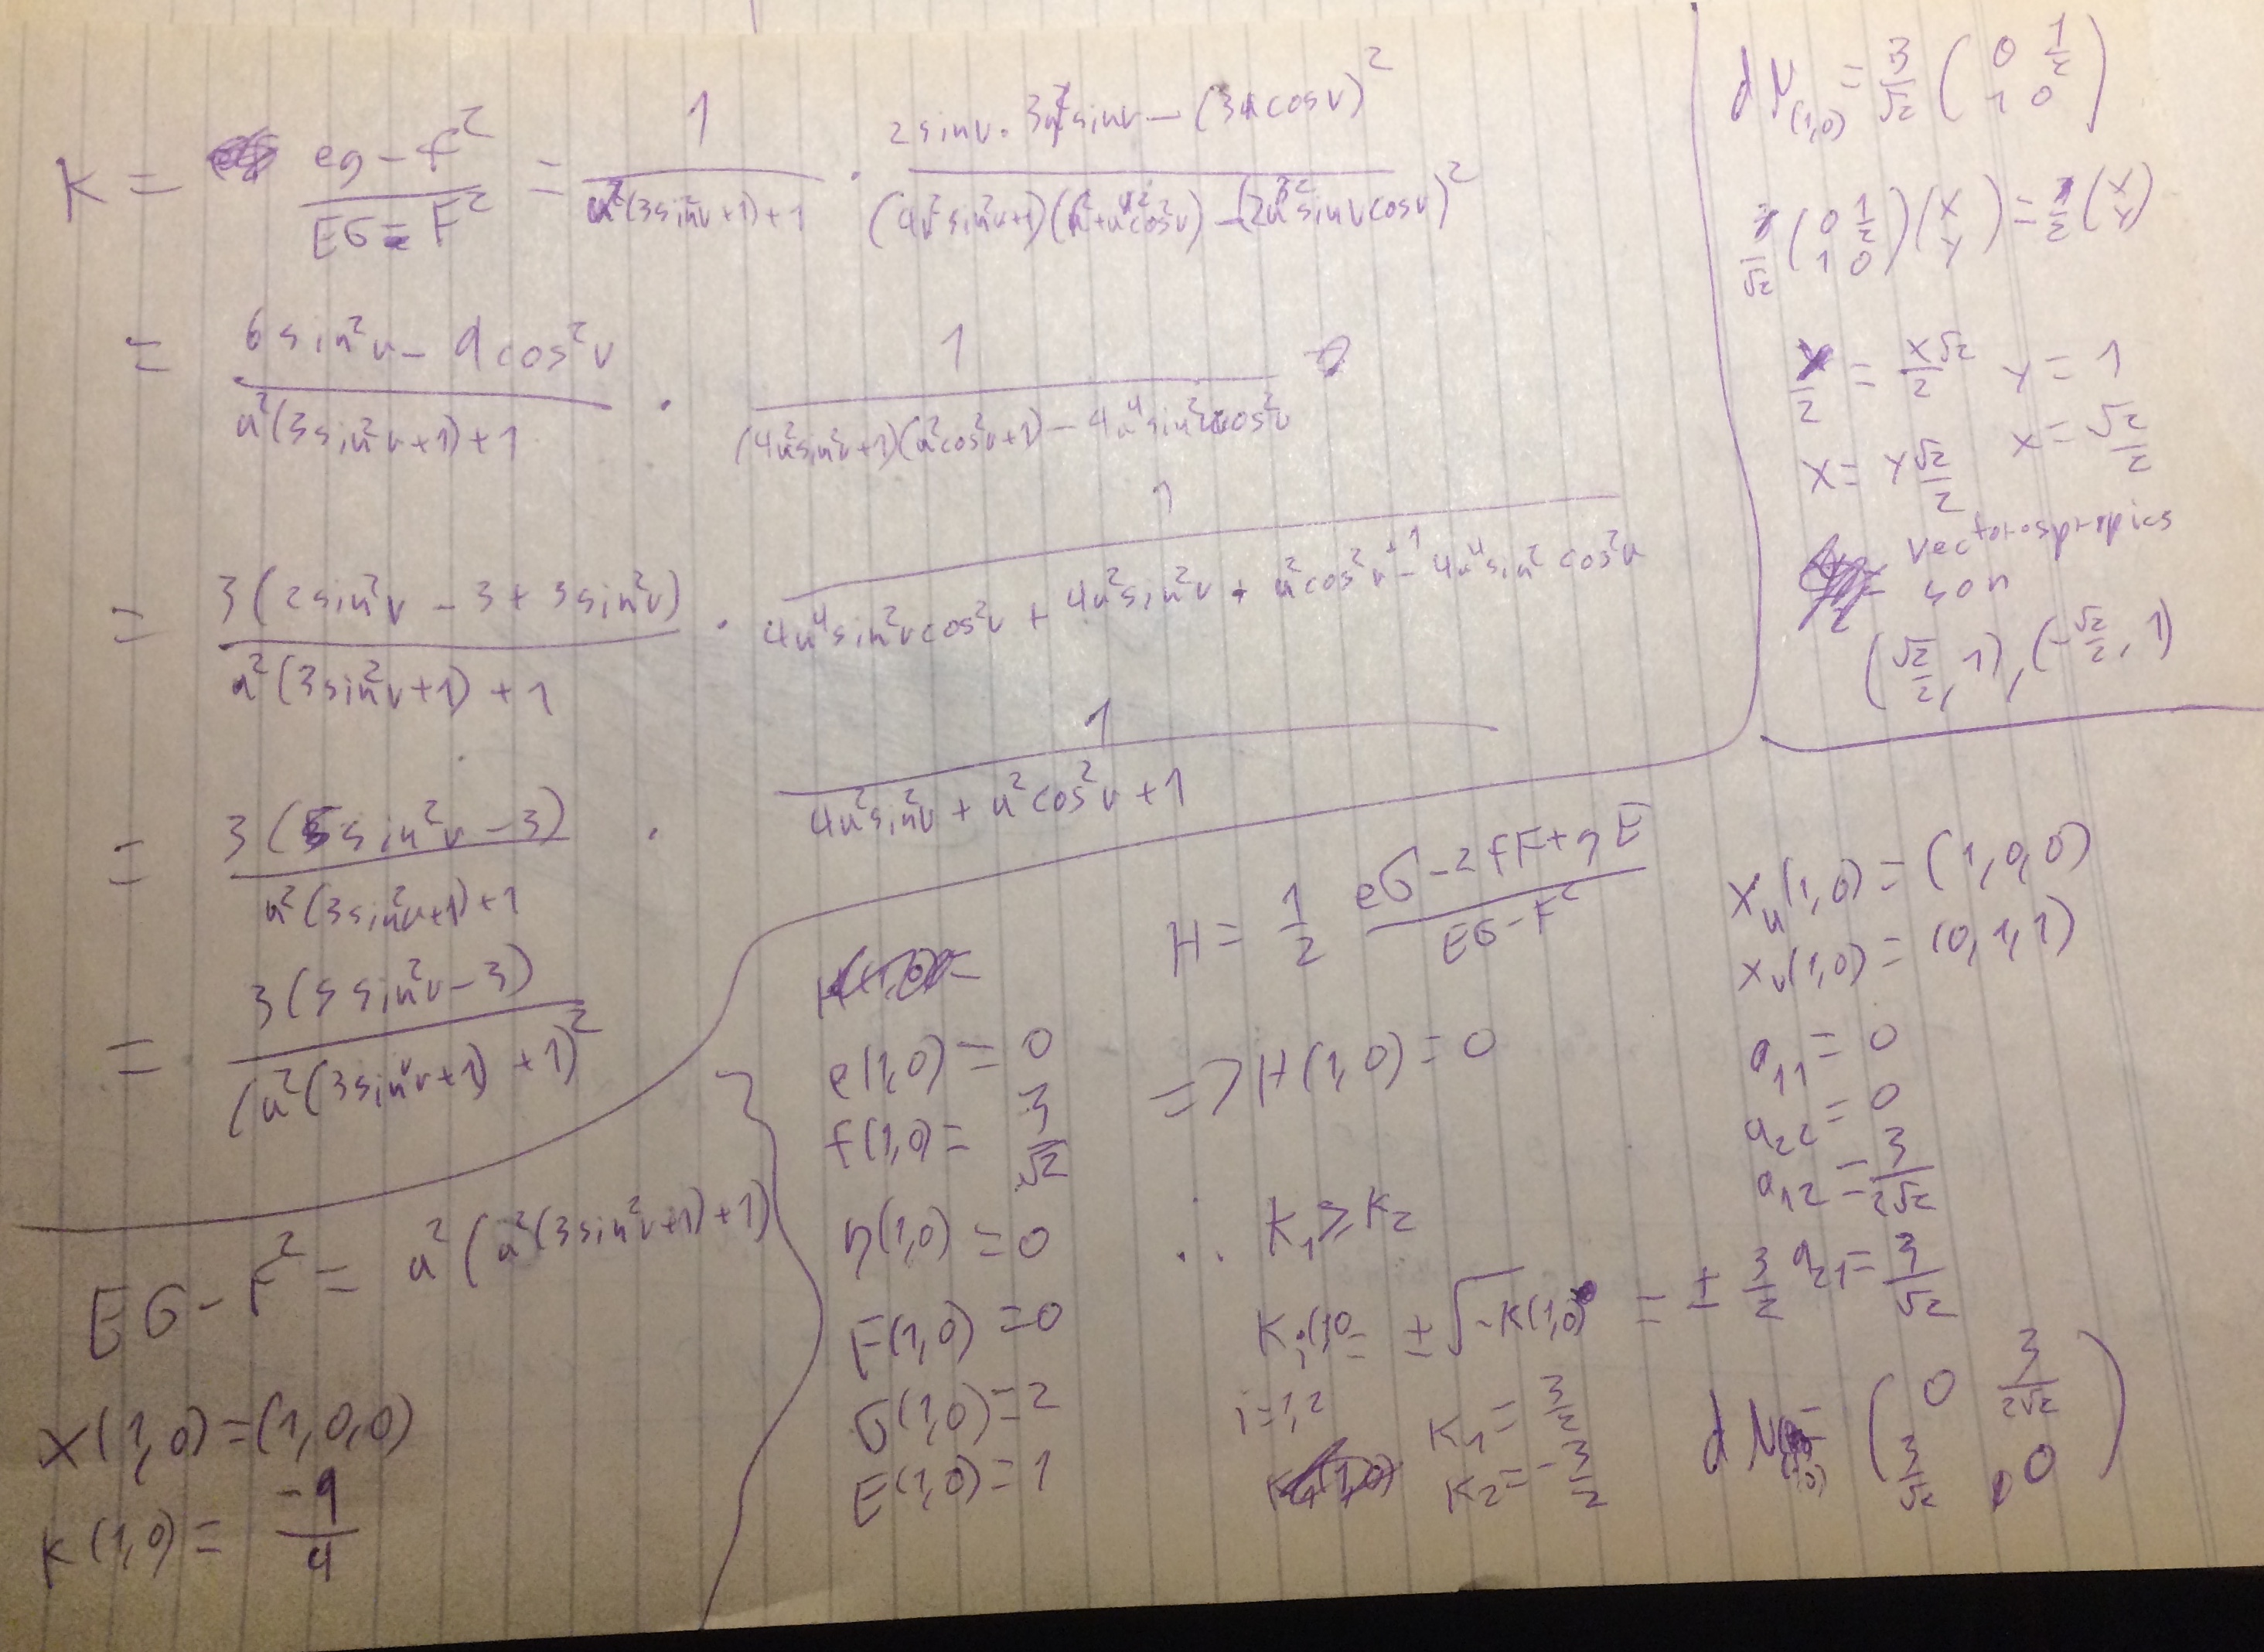
\includegraphics{img/IMG_5985.JPG}
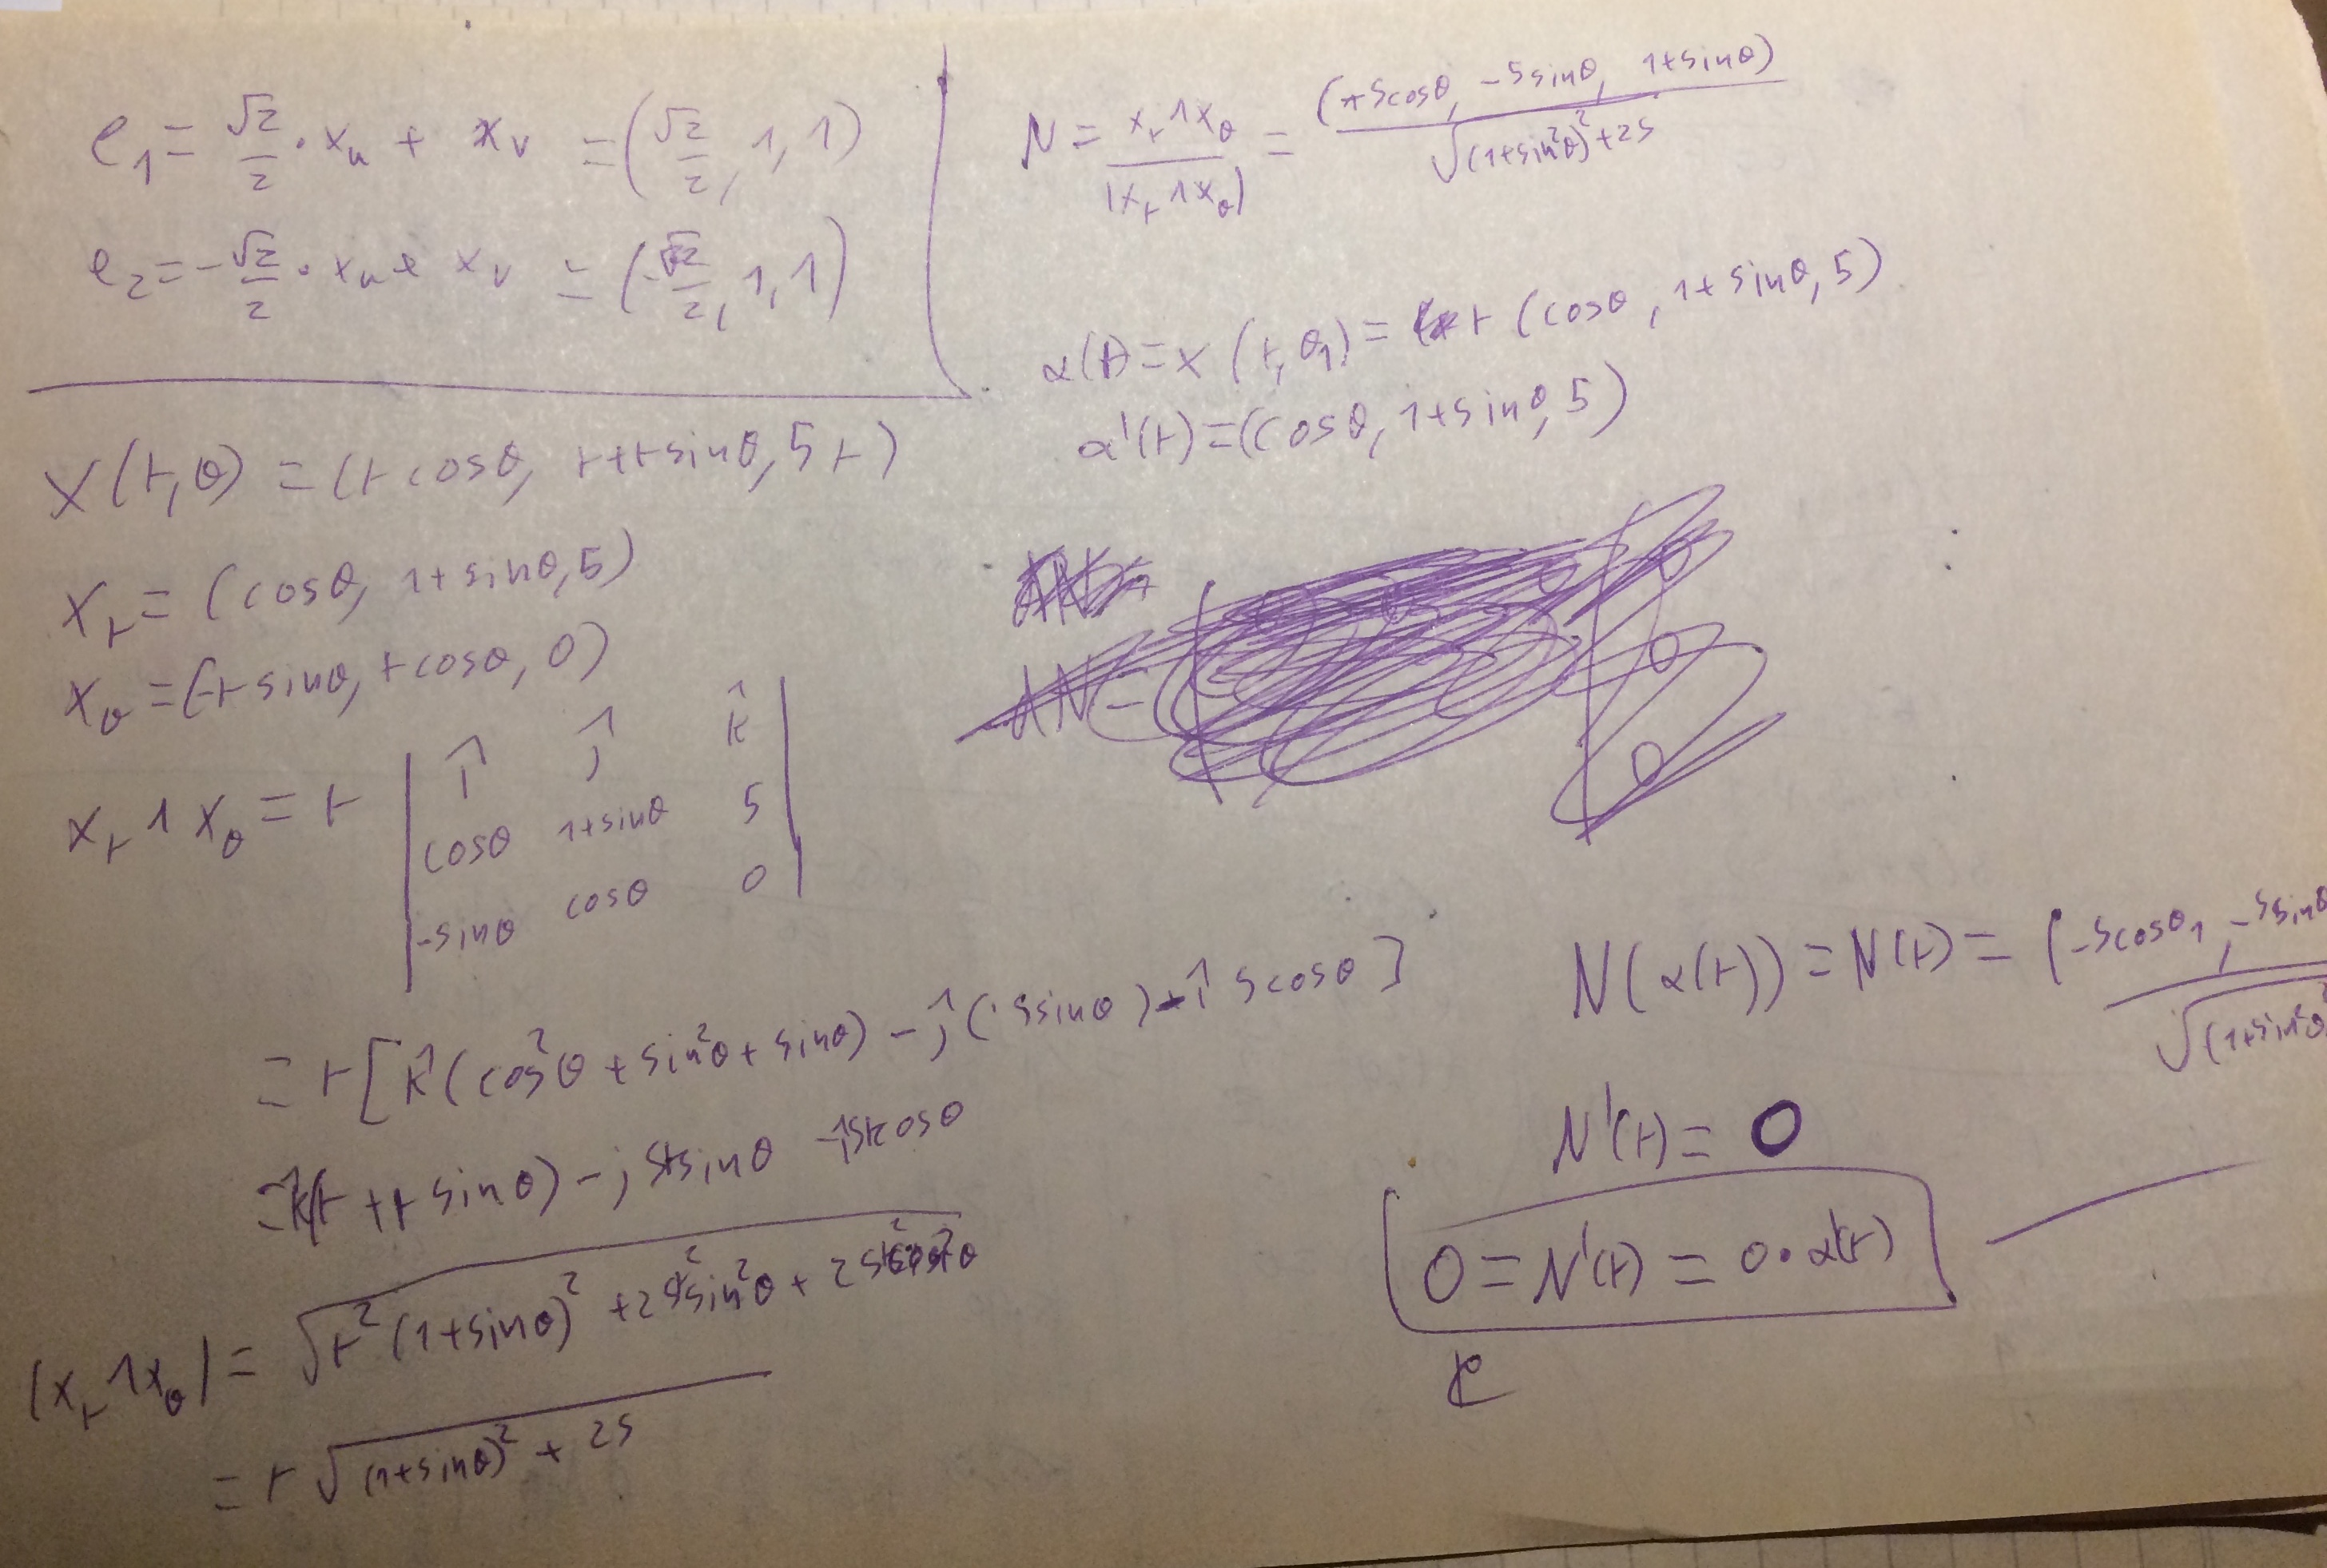
\includegraphics{img/IMG_5986.JPG}
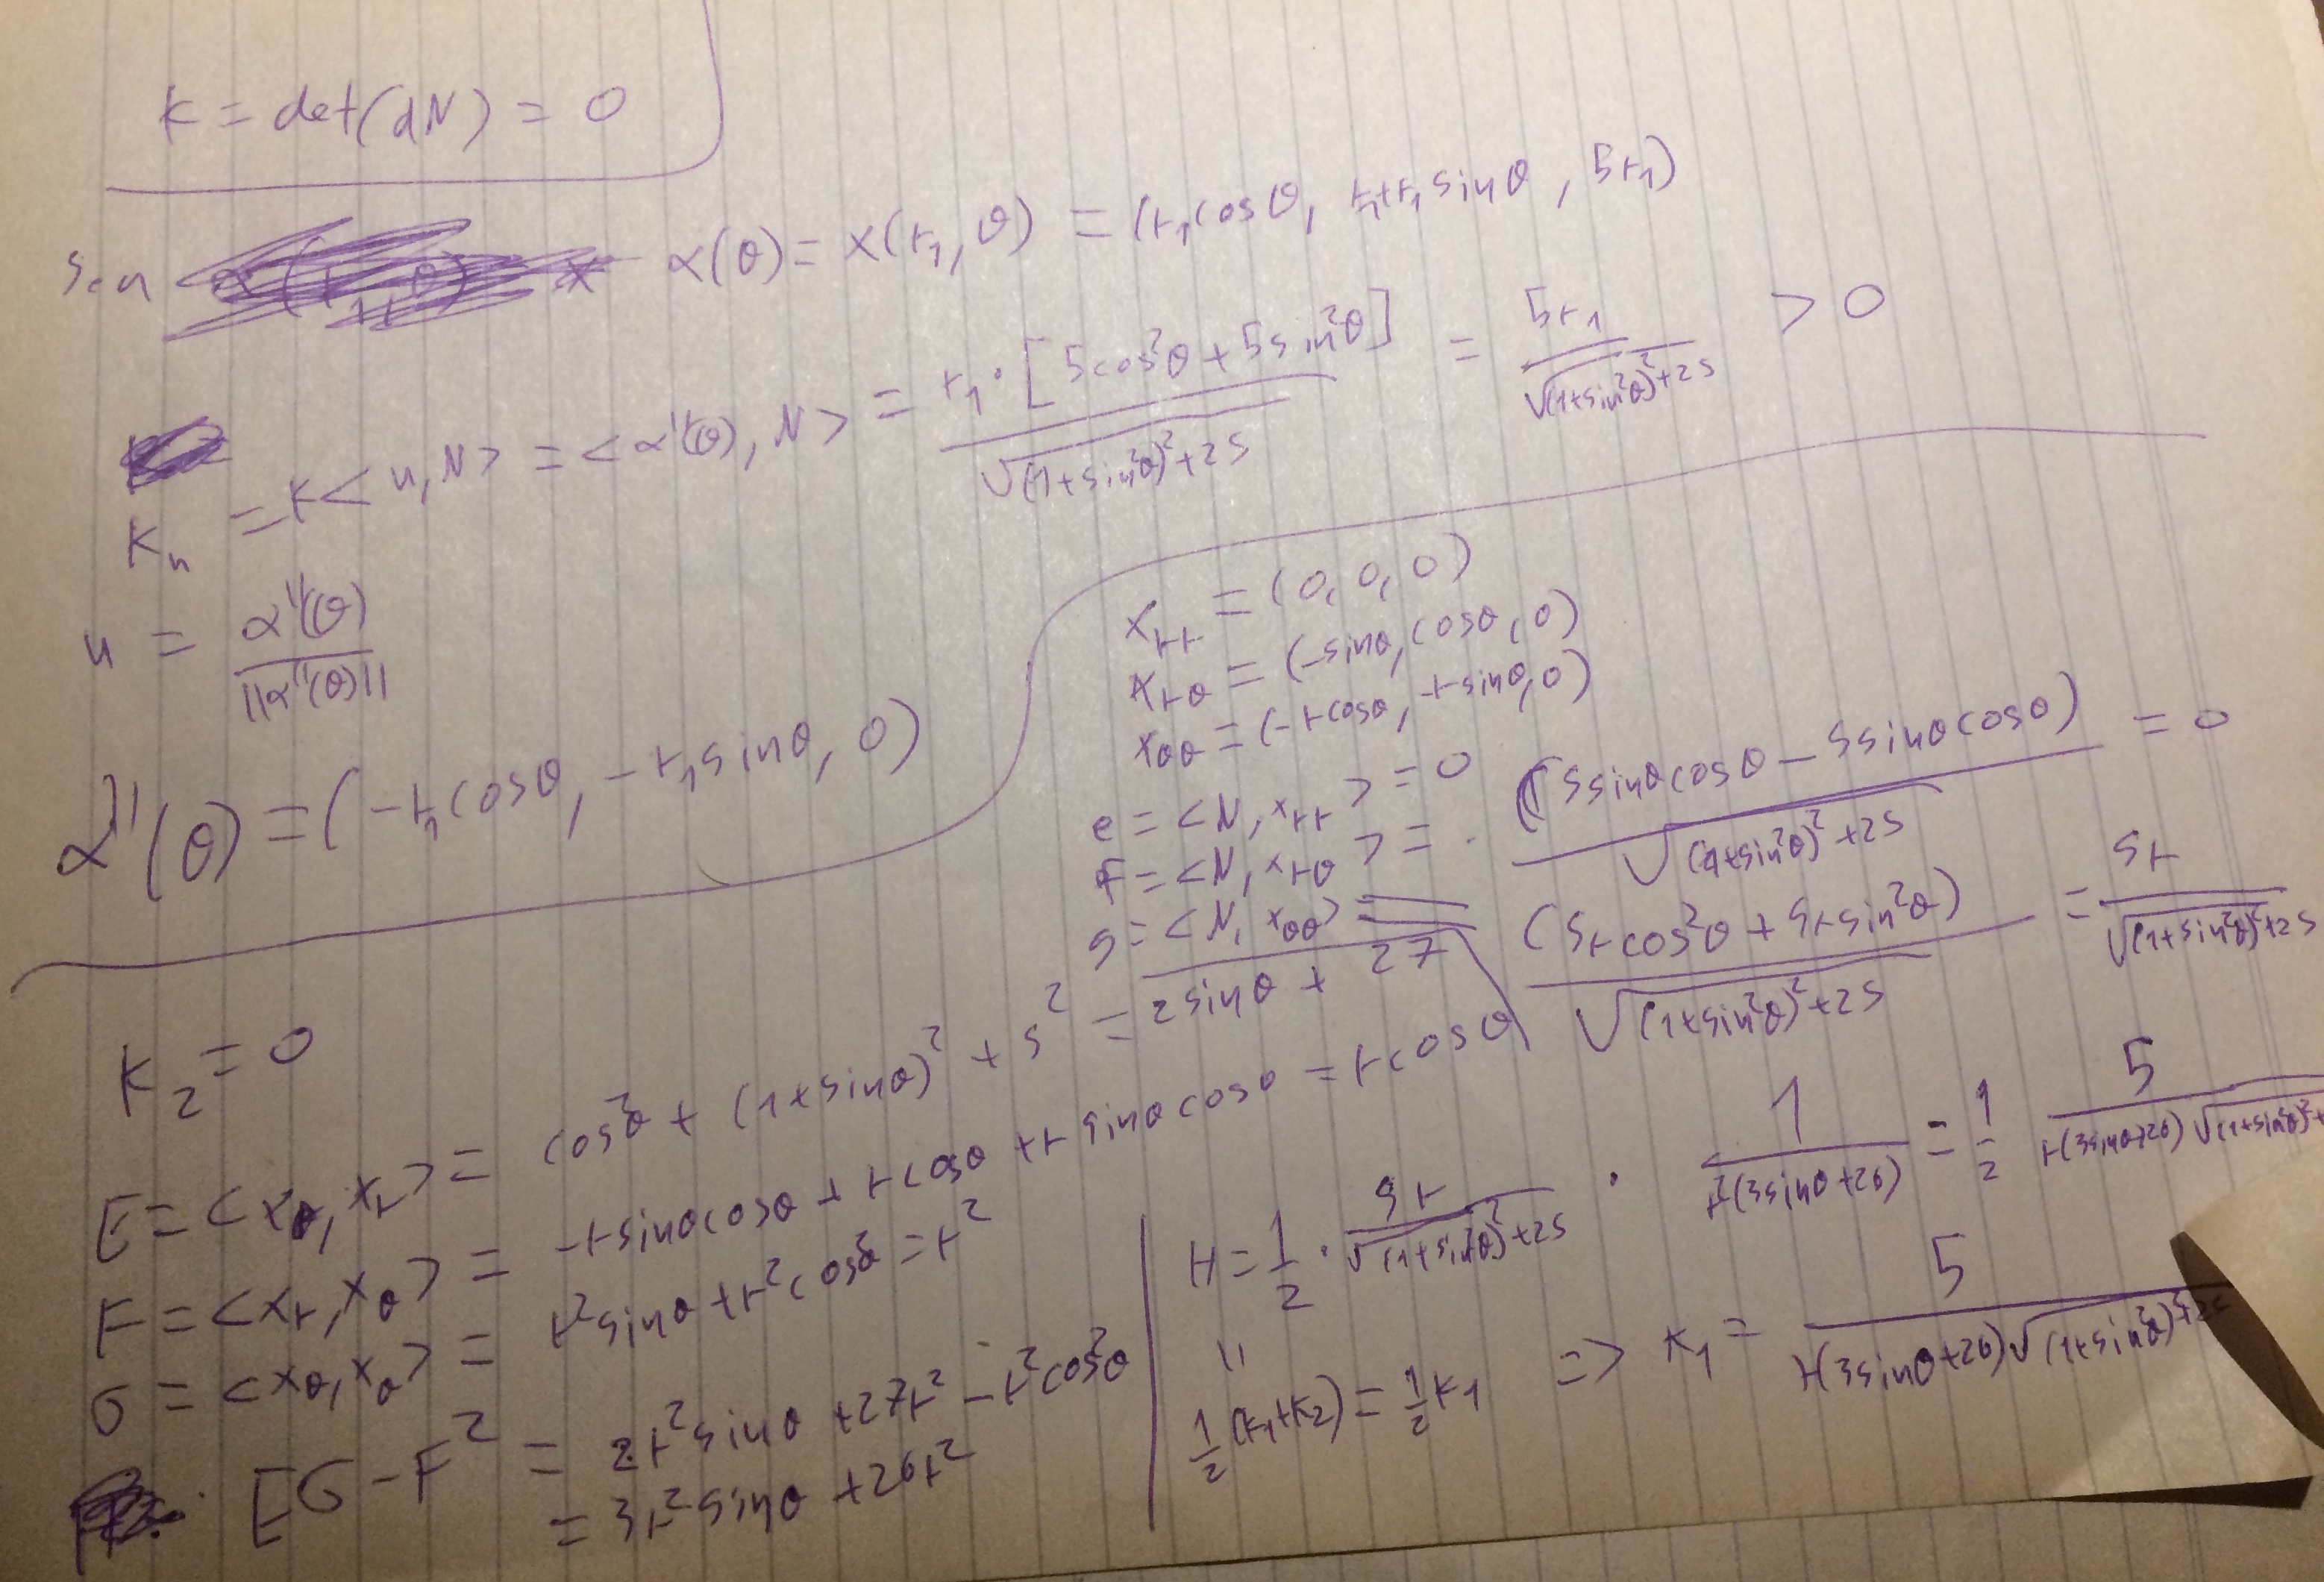
\includegraphics{img/IMG_5987.JPG}
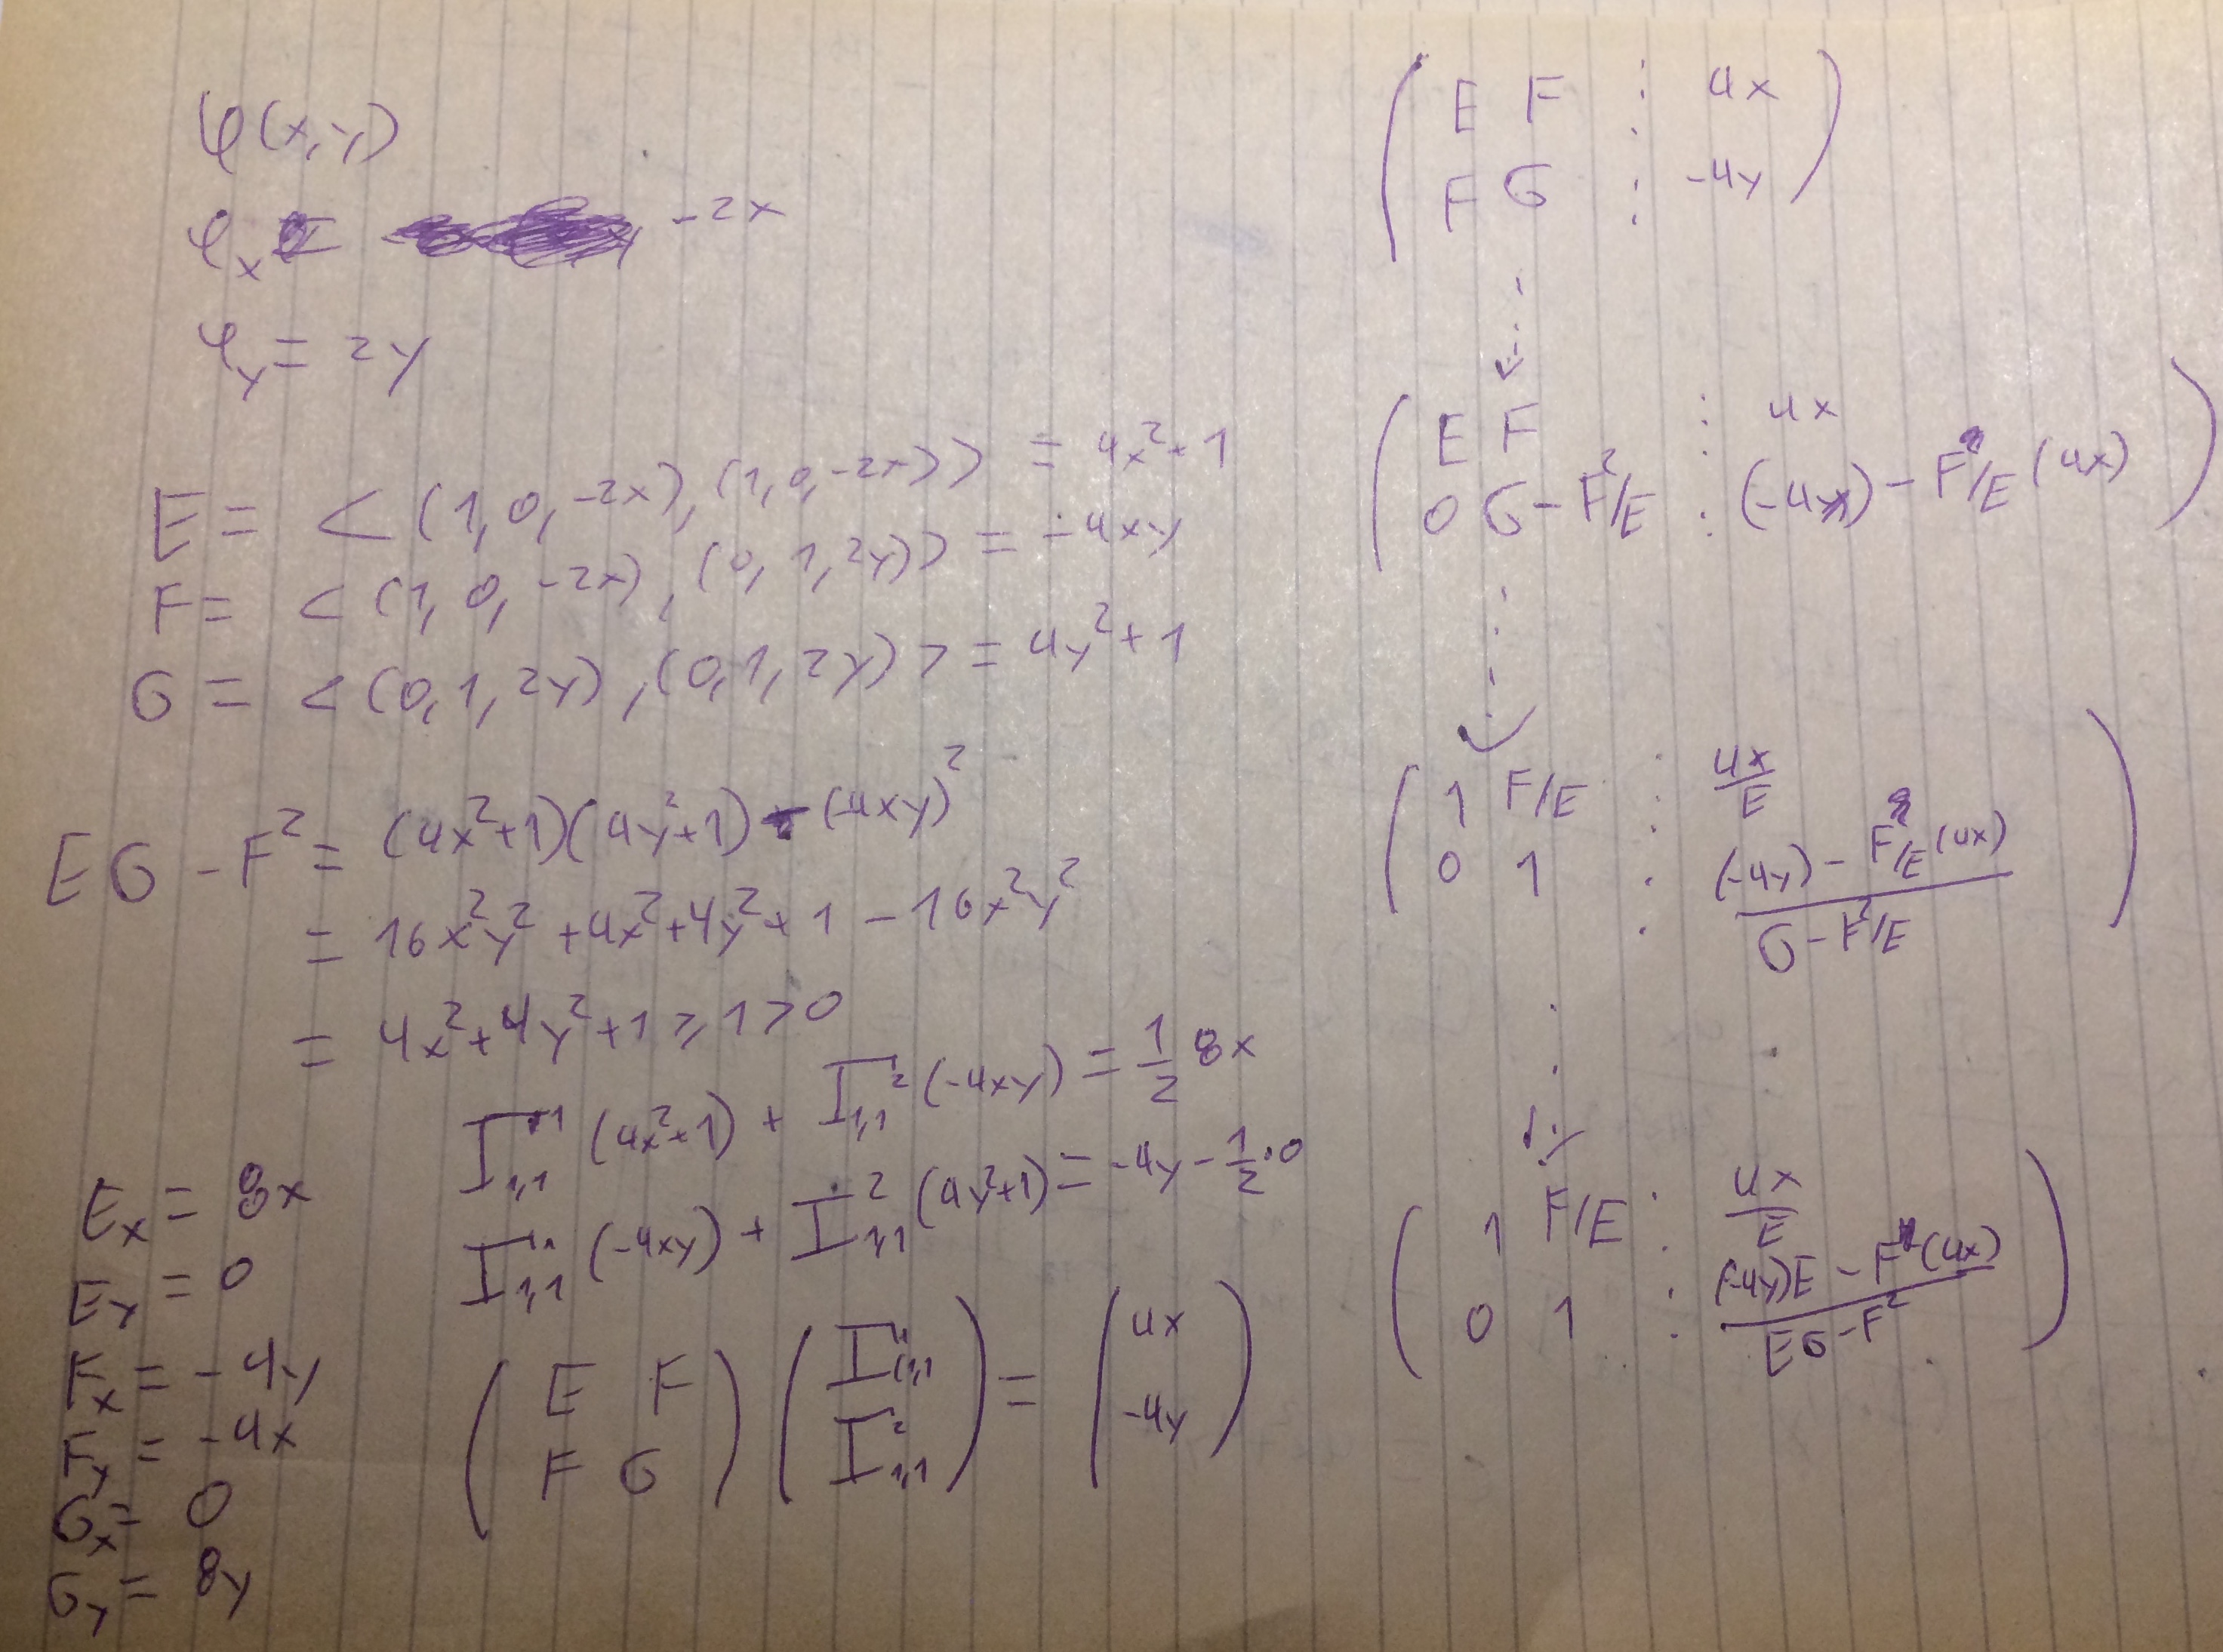
\includegraphics{img/IMG_5988.JPG}
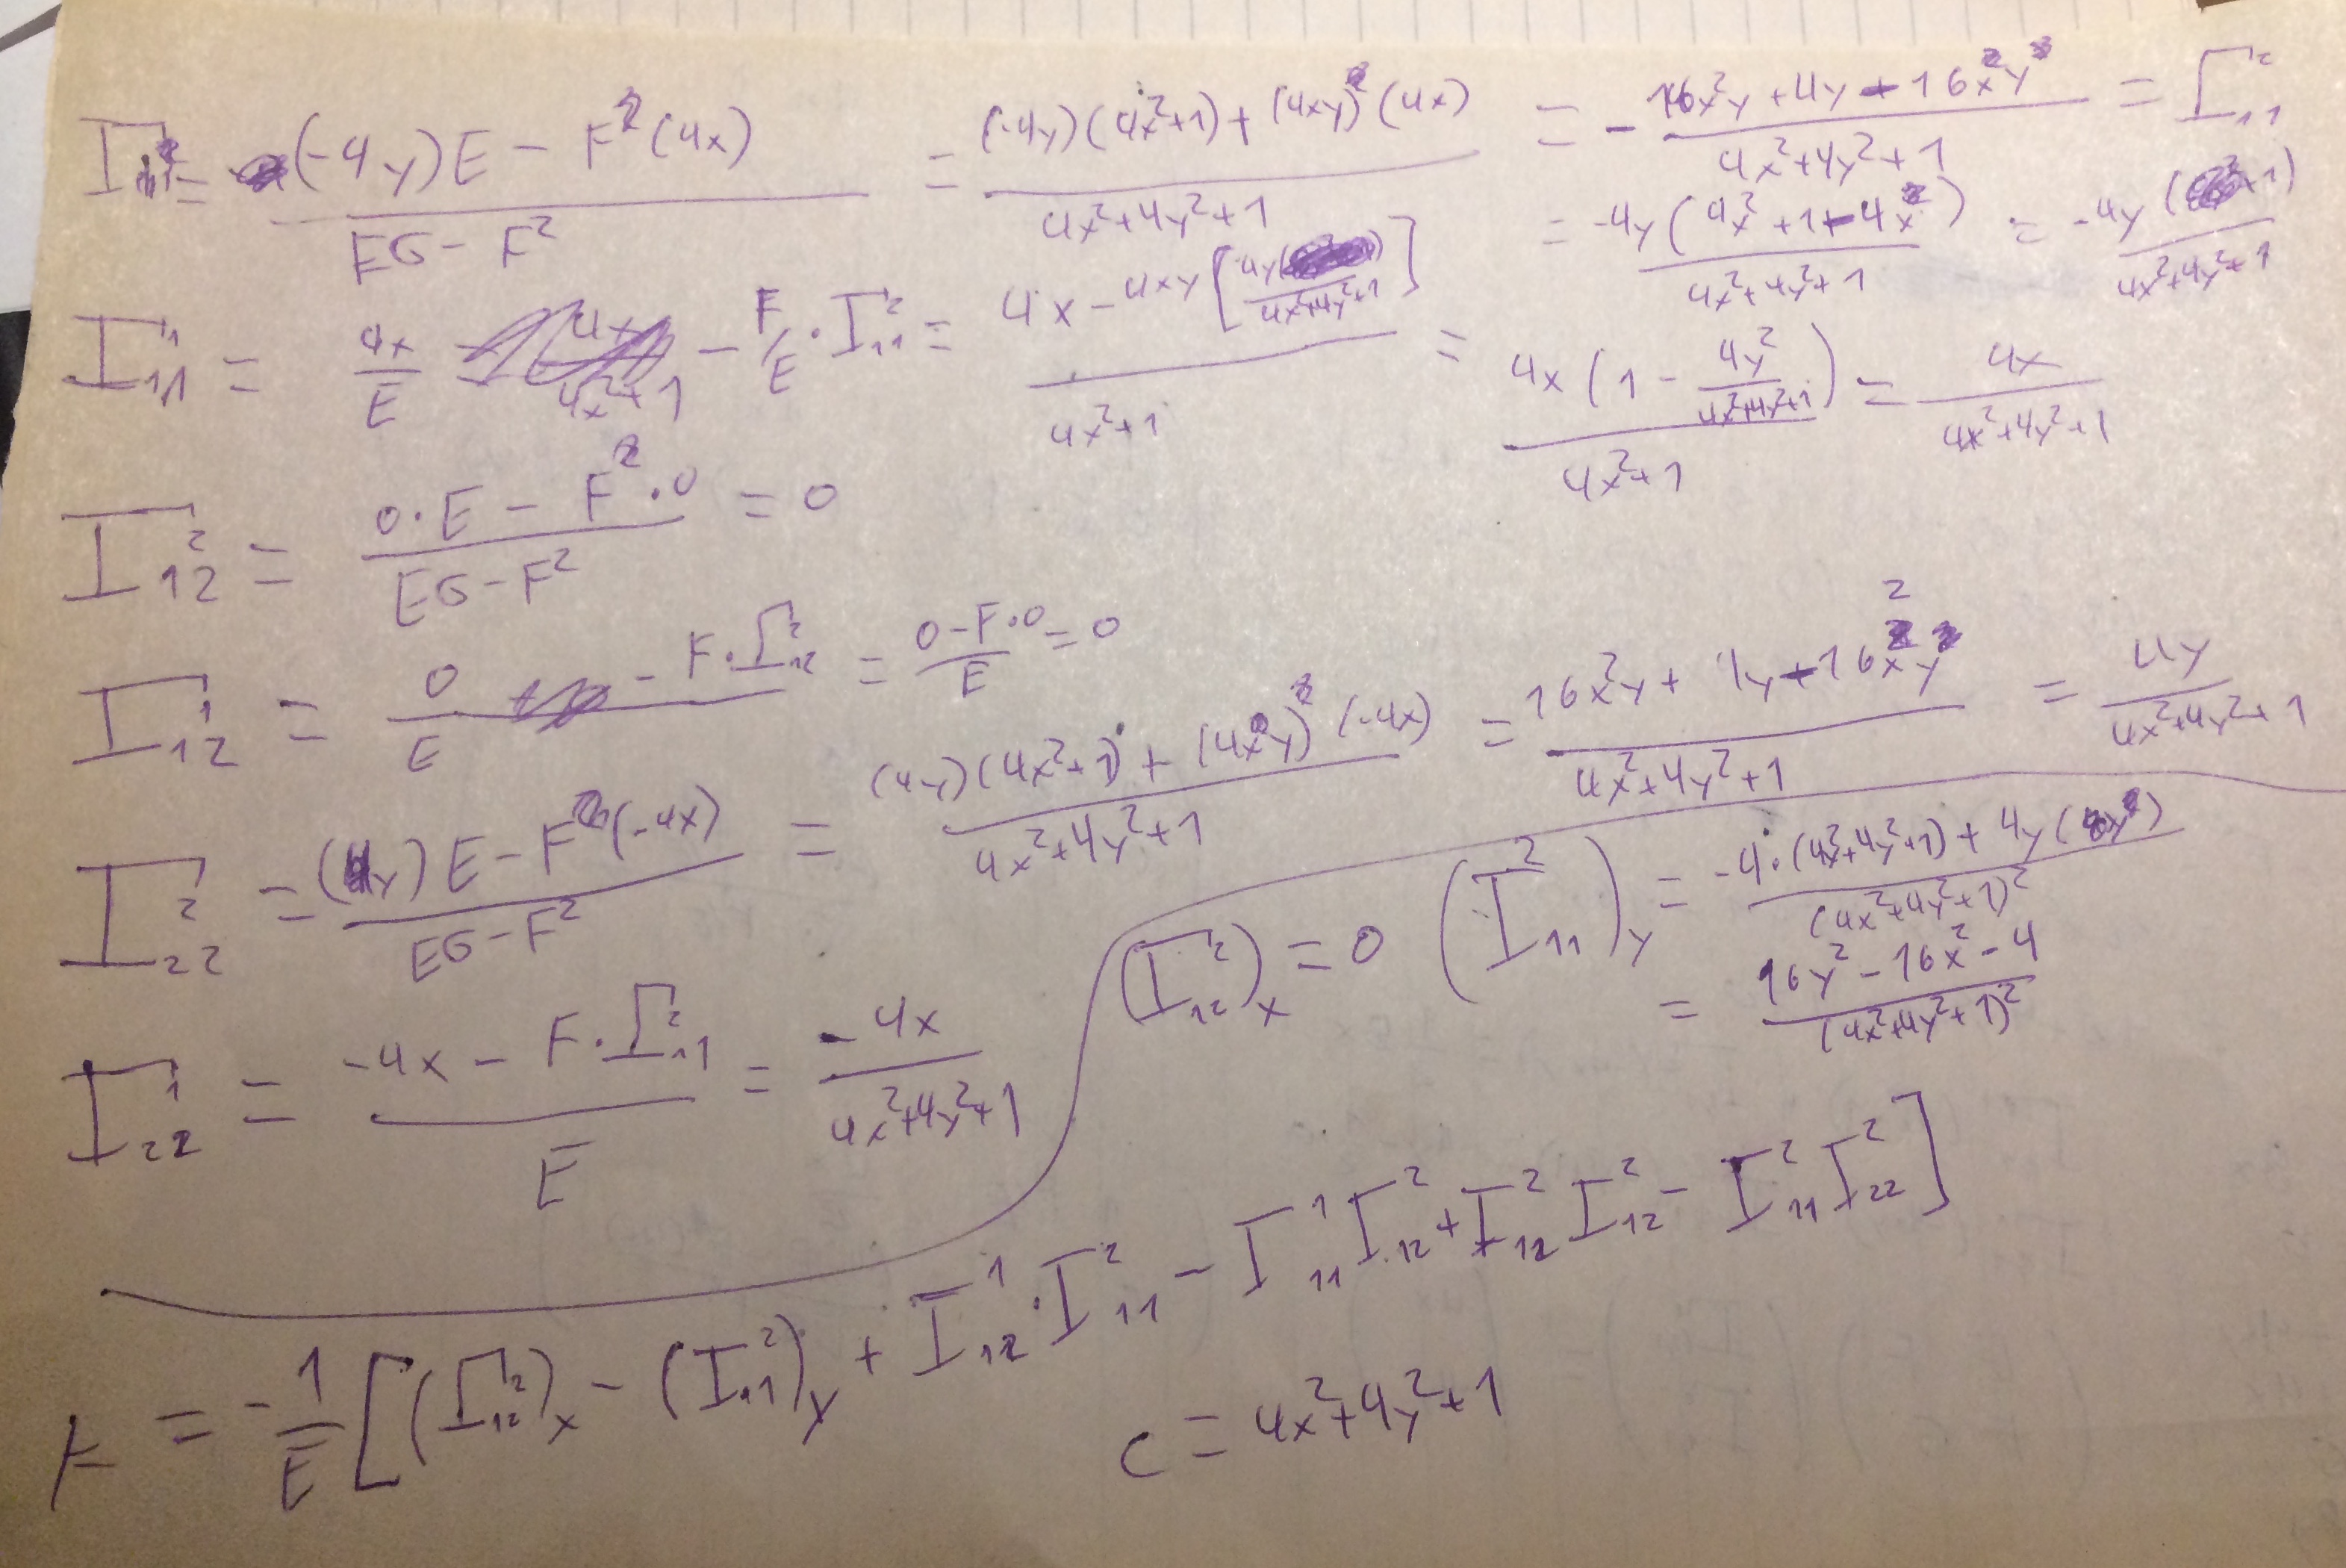
\includegraphics{img/IMG_5989.JPG}
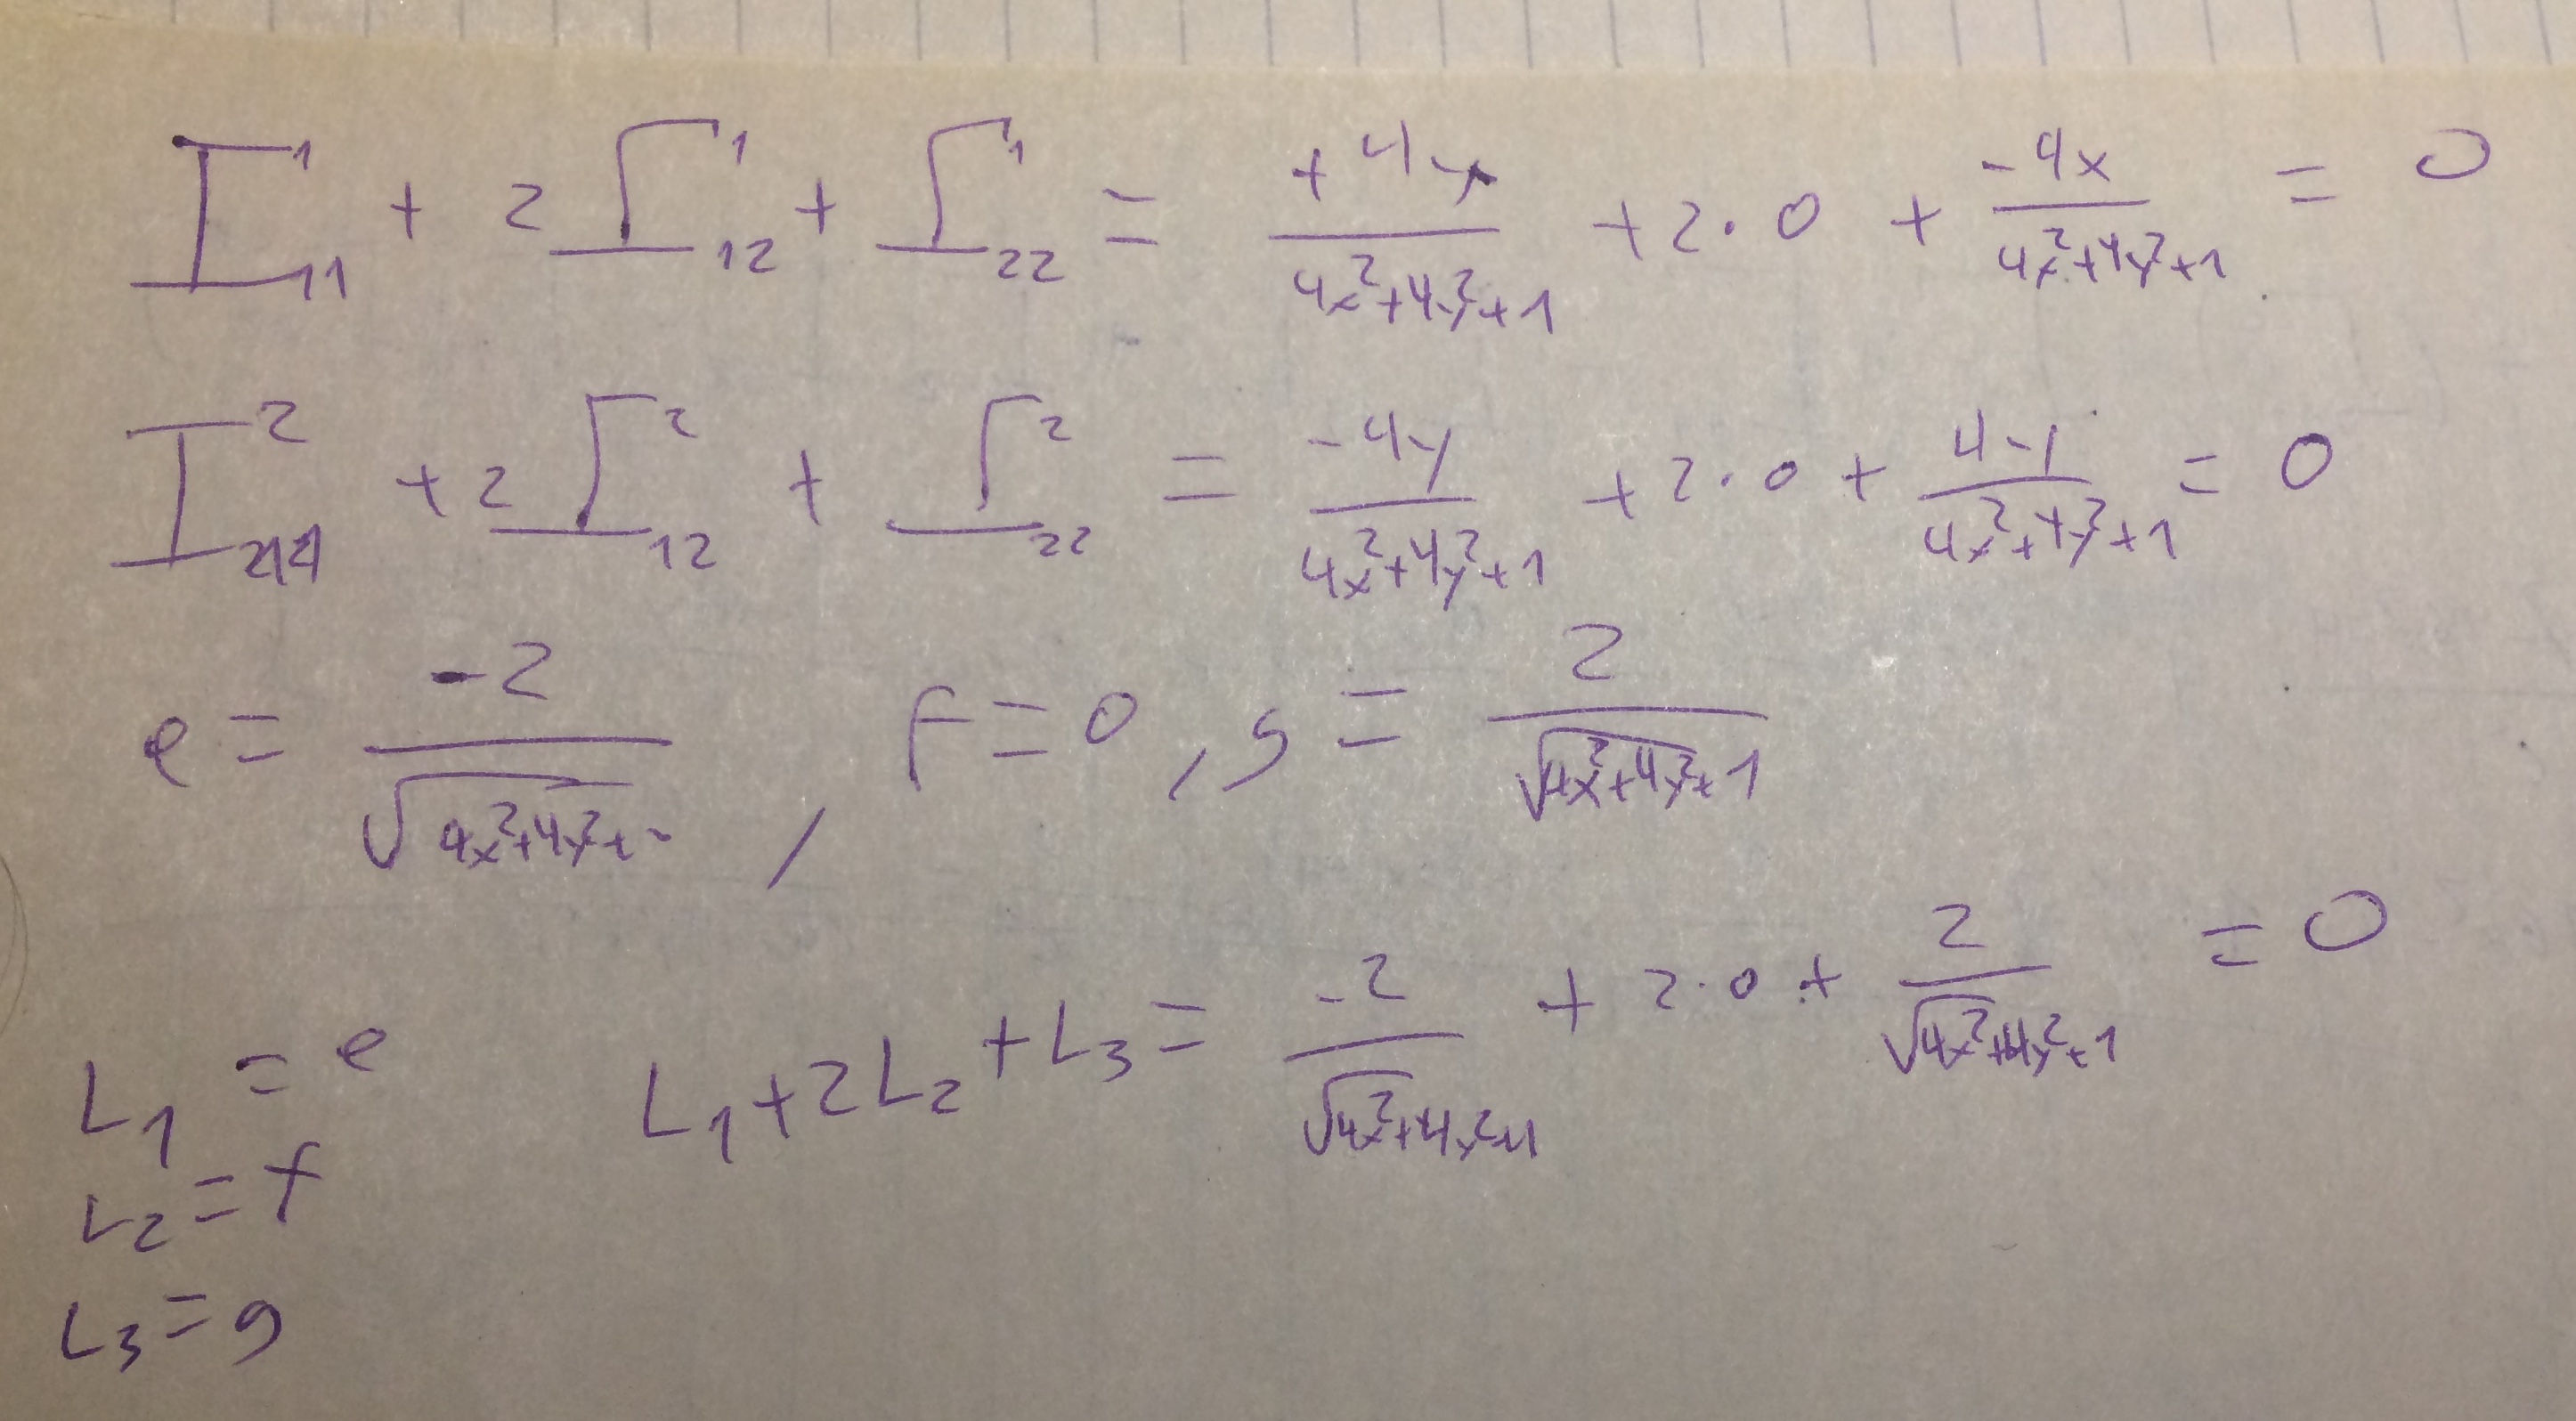
\includegraphics{img/IMG_5990.JPG}
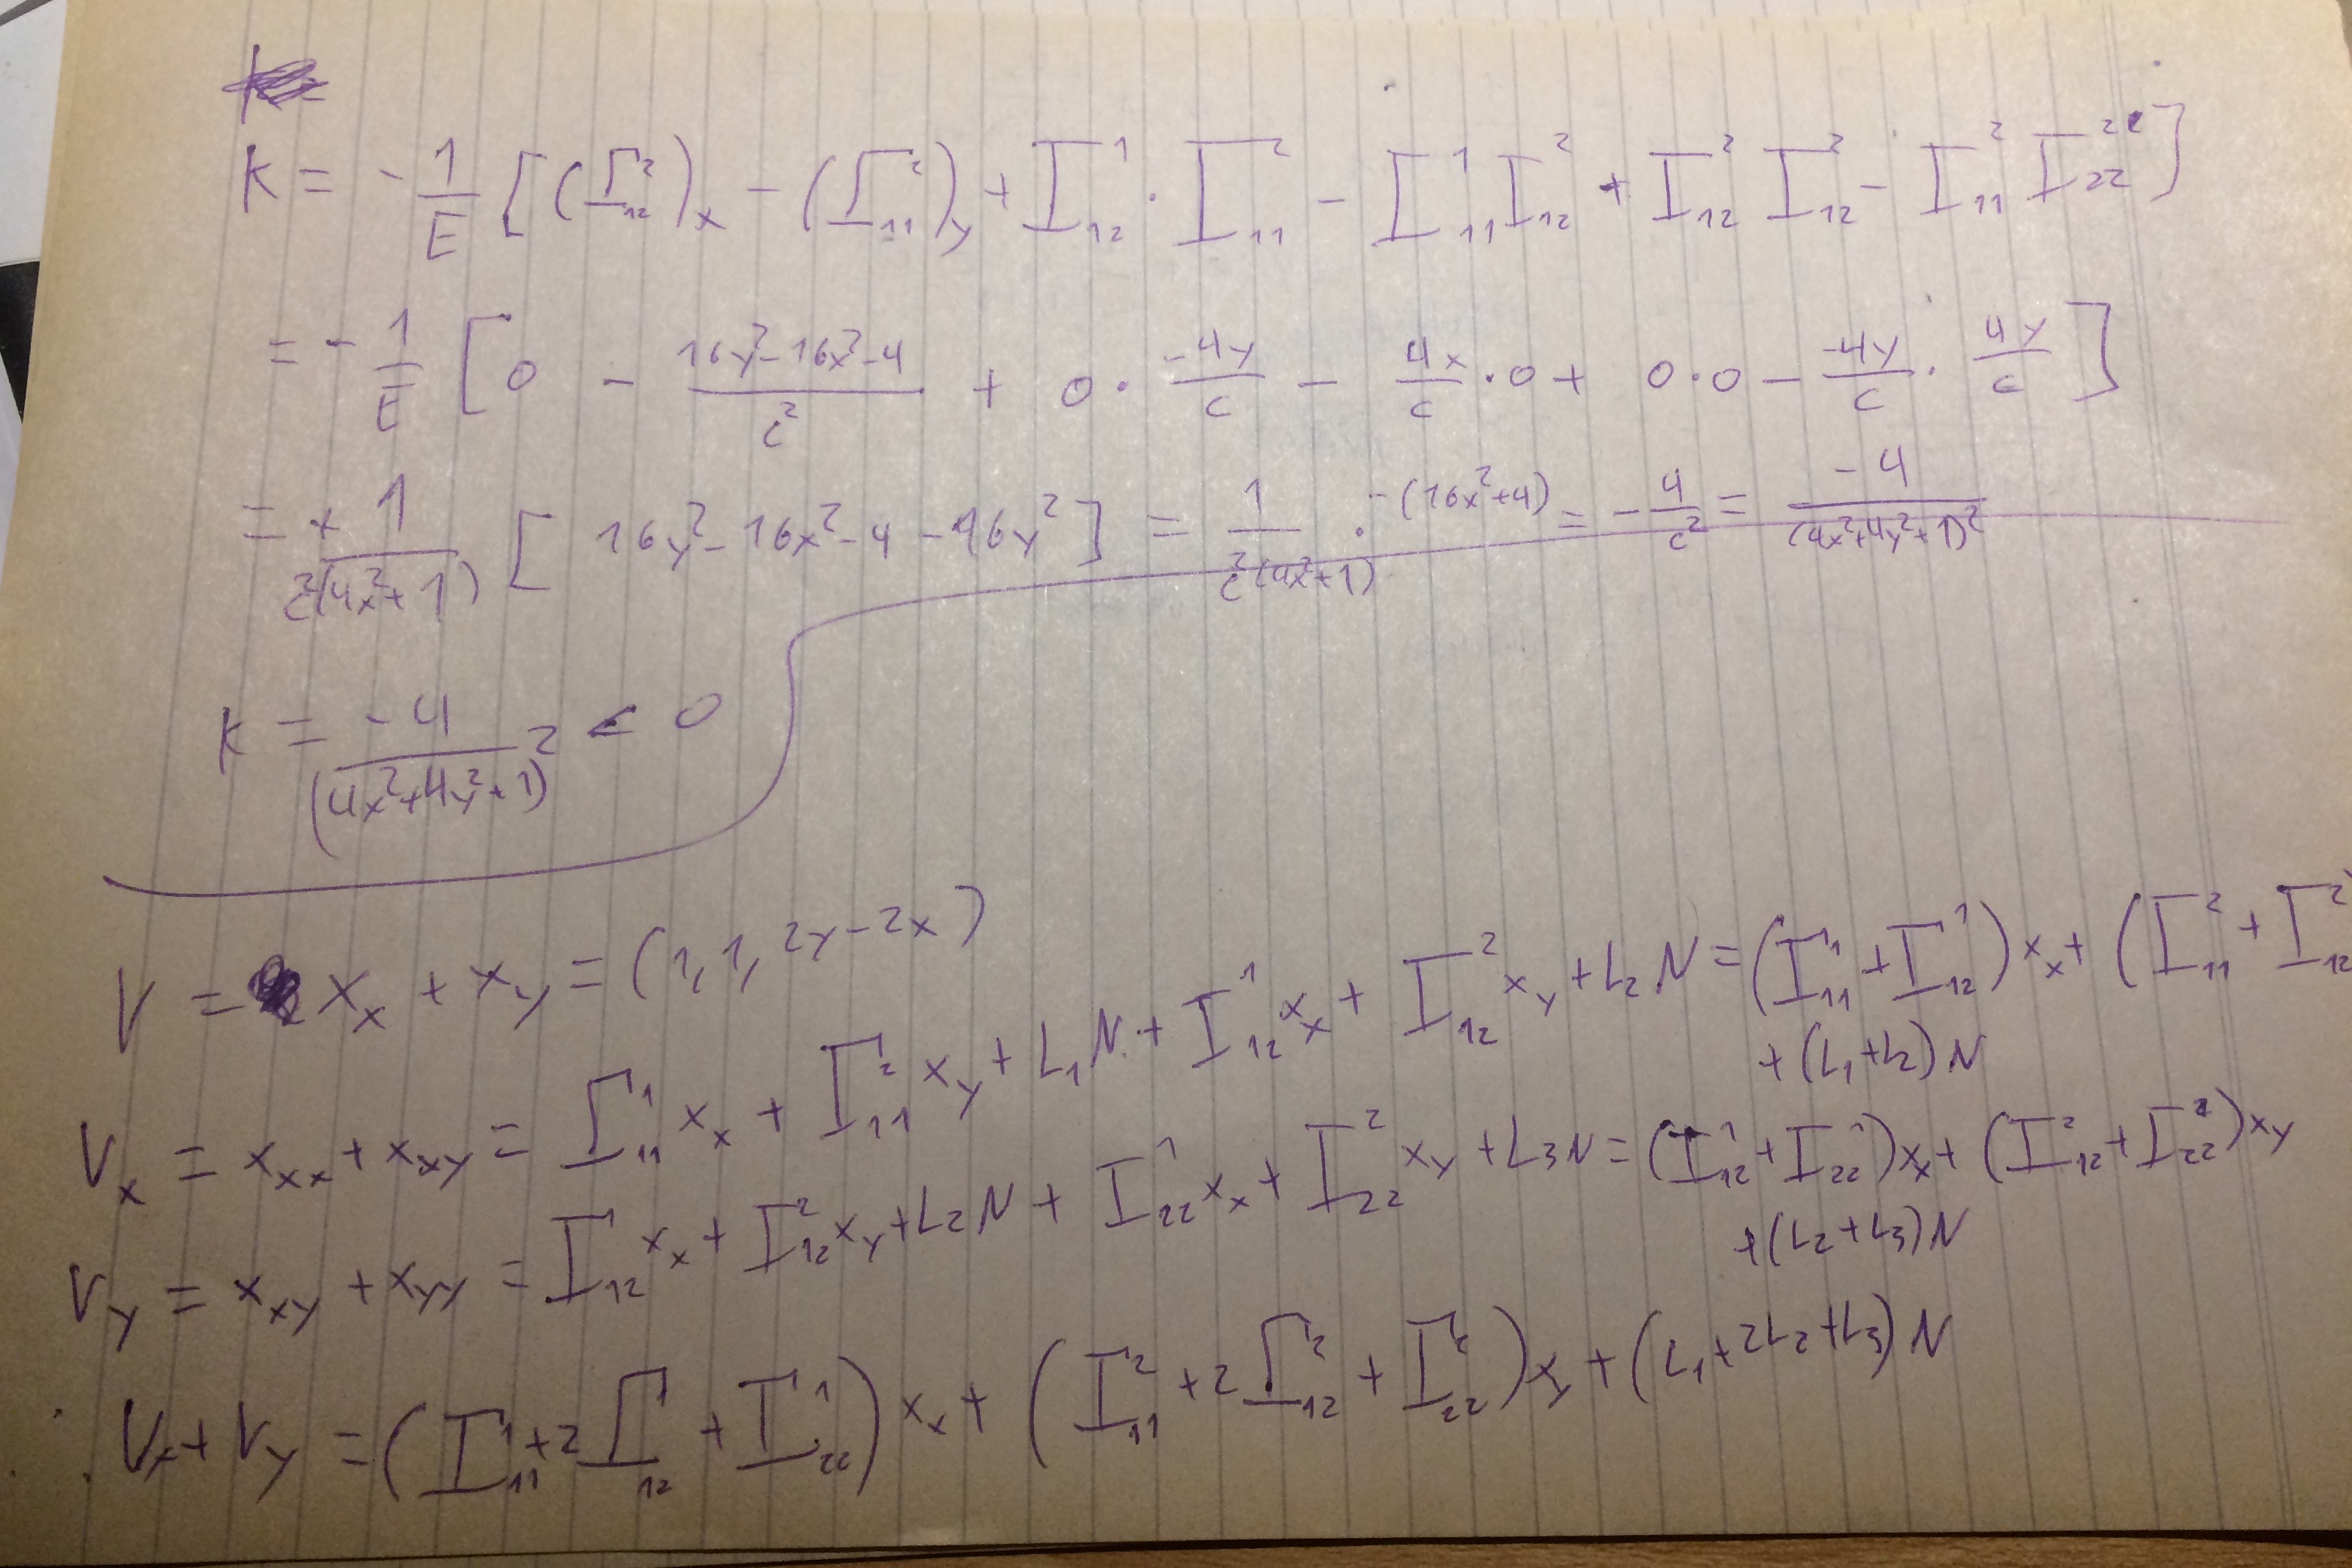
\includegraphics{img/IMG_5991.JPG}

\end{center}
\end{document}